\documentclass[
    11pt, % Set the default font size, options include: 8pt, 9pt, 10pt, 11pt, 12pt, 14pt, 17pt, 20pt
    %
    aspectratio=169, % Uncomment to set the aspect ratio to a 16:9 ratio which matches the aspect ratio of 1080p and 4K screens and projectors
]{beamer}

\graphicspath{{Images/}{./}} % Specifies where to look for included images (trailing slash required)
\usepackage{booktabs} % Allows the use of \toprule, \midrule and \bottomrule for better rules in tables

%\usepackage{appendixnumberbeamer} %If you want a separate slide counter for your appendix

%%% Customize Theme %%%%%%%%%%%%%%%%%%%%%%
\usetheme{Madrid} % You can use other themes too, but this changes many things. I've found Madrid to be the best for this color scheme

%fg = font color
%bg = background color

% ! WARNING ! : Many colors are linked to multiple attributes, so changing one color can have unexpected changes!

% If you want to tweak the shading of colors, tweak the below 2 lines:
\definecolor{myBlue}{RGB}{50, 148, 109}
\definecolor{myTeal}{RGB}{229, 61, 0}

% Bottom right hand color
\setbeamercolor*{structure}{bg=myBlue,fg=myBlue}

\setbeamercolor*{palette primary}{use=structure,fg=white,bg=structure.fg} %?
\setbeamercolor*{palette secondary}{use=structure,fg=myBlue,bg=white}
    %bottom left of footer & bar between title & top bubbles
\setbeamercolor*{palette tertiary}{use=structure,fg=white,bg=myBlue}

\setbeamercolor{frametitle}{bg=myBlue,fg=white} %title of each slide

\setbeamercolor*{titlelike}{parent=palette primary} %?
%\setbeamercolor{titlelike}{parent=palette primary,fg=structure.fg!50!myBlue}

%for miniframe (very top) AND center footer
\setbeamercolor{section in head/foot}{fg=myTeal, bg=white}

%%% Specific Colors %%%
\setbeamercolor{item projected}{bg=myTeal}
\setbeamertemplate{enumerate items}{bg=myTeal}

\setbeamercolor{itemize item}{fg=myTeal}
\setbeamercolor{itemize subitem}{fg=myTeal}

\setbeamercolor{button}{bg=myTeal}

%%% Edits ONLY the TOC slide %%%
\setbeamercolor{section in toc}{fg=black}
\setbeamercolor{subsection in toc}{fg=black}

%%% Block Colors %%%
% Standard block %
    \setbeamercolor{block title}{bg=myTeal, fg=white}
    \setbeamercolor{block body}{bg=myTeal!20}

% Alerted block % If you want to customize it's color
    %\setbeamercolor{block title alerted}{bg=cyan, fg=white}
    %\setbeamercolor{block body alerted}{bg=cyan!10}

% Example block % If you want to customize it's color
    %\setbeamercolor{block title example}{bg=cyan, fg=white}
    %\setbeamercolor{block body example}{bg=cyan!10}

%---------------------------------------------------------
%	SELECT FONT THEME & FONTS
%---------------------------------------------------------
\usefonttheme{professionalfonts}
\usepackage{iftex}
\ifPDFTeX
  \usepackage[T1]{fontenc}
  \usepackage{newtxtext}
  \usepackage{newtxmath}
\else
  \usepackage{fontspec}
  \setmainfont{Times New Roman}
  \setsansfont{Times New Roman}
  \setmonofont{Courier New}
\fi
% Added math + TikZ
\usepackage{amsmath}
\usepackage{tikz}
\usepackage{relsize}
\usepackage{array}     % For advanced column formatting like >{\centering\arraybackslash}
\usepackage{multirow}  % For multirow cells in tables
\tikzset{>=latex} % for LaTeX arrow head
\colorlet{myred}{red!80!black}
\colorlet{myblue}{blue!80!black}
\colorlet{mygreen}{green!60!black}
\colorlet{mydarkred}{myred!40!black}
\colorlet{mydarkblue}{myblue!40!black}
\colorlet{mydarkgreen}{mygreen!40!black}
\colorlet{myorange}{orange!80!black}
\colorlet{myviolet}{blue!50!red!60}
\tikzstyle{node}=[very thick,circle,draw=myblue,minimum size=22,inner sep=0.5,outer sep=0.6]
\tikzstyle{connect}=[->,thick,mydarkblue,shorten >=1]
\tikzset{ % node styles, numbered for easy mapping with \nstyle
  node 1/.style={node,mydarkgreen,draw=mygreen,fill=mygreen!25},
  node 2/.style={node,mydarkblue,draw=myblue,fill=myblue!20},
  node 3/.style={node,mydarkred,draw=myred,fill=myred!20},
}
\def\nstyle{int(\lay<\Nnodlen?min(2,\lay):3)} % map layer number onto 1, 2, or 3

\usetikzlibrary{arrows.meta,shadows,positioning}
\usepackage{listofitems} 
\usetikzlibrary{calc}
\usetikzlibrary{fit, positioning, shapes.geometric}
\tikzset{
	frame/.style={
		rectangle, draw,
		text width=6em, text centered,
		minimum height=4em,drop shadow,fill=white,
		rounded corners,
	},
	line/.style={
		draw, -{Latex},rounded corners=3mm,
	}
}
\usetikzlibrary{arrows.meta,positioning,calc,decorations.pathmorphing}
\usepackage{subcaption} % added for side-by-side subfigures
\pgfmathsetmacro{\r}{0.8}
\pgfmathsetmacro{\Phi}{-160}
\pgfmathsetmacro{\Theta}{-90}
\usepackage{fontawesome5}
\usepackage{float}
\usepackage{amsmath}
\usepackage{physics}
\usepackage{algorithm, algorithmic}
\usetikzlibrary{arrows.meta,positioning,calc,decorations.pathmorphing}

\useinnertheme{circles}

%---------------------------------------------------------
%	SELECT OUTER THEME
%---------------------------------------------------------
% Outer themes change the overall layout of slides, such as: header and footer lines, sidebars and slide titles. Uncomment each theme in turn to see what changes it makes to your presentation.

%\useoutertheme{default}
%
\useoutertheme{miniframes}

% \useoutertheme{infolines}
% \useoutertheme{smoothbars}
% \useoutertheme{sidebar}
% \useoutertheme{split}
% \useoutertheme{shadow}
% \useoutertheme{tree}
% \useoutertheme{smoothtree}

%---------------------------------------------------------
%	PRESENTATION INFORMATION
%---------------------------------------------------------

\title[Multi-Agent RL for Spacecraft Guidance]{Robust Reinforcement Learning Differential Game Guidance in Low-Thrust, Multi-Body Dynamical Environments}
\subtitle{A Zero-Sum Reinforcement Learning Approach in Three-Body Dynamics}
\author[Ali Baniasad]{Ali Baniasad \\ \smallskip Supervisor: Dr. Nobahari}

\institute[]{Department of Aerospace Engineering \\ \smallskip Sharif University of Technology}
\date[\today]

\logo{\includegraphics[width=.75cm]{sharif_logo.png}}

%---------------------------------------------------------
%---------------------------------------------------------
%---------------------------------------------------------
\begin{document}

%---------------------------------------------------------
%	TITLE SLIDE
%---------------------------------------------------------
\section{}
\begin{frame}
	\titlepage % Output the title slide, automatically created using the text entered in the PRESENTATION INFORMATION block above

\end{frame}

%---------------------------------------------------------
%	TABLE OF CONTENTS SLIDE
%---------------------------------------------------------

\begin{frame}
	\frametitle{Outline}
	\tableofcontents
\end{frame}

% --- Chapters added from report ---
\section{Introduction \& Motivation}

% %------------------------------------------------
\begin{frame}
    \frametitle{Research Motivation}
    \vspace{-0.5cm}

    % \begin{exampleblock}{Key Motivation Drivers}
    \begin{itemize}
        \item \textbf{Space missions} increasingly require autonomous guidance systems
        \item \textbf{Low-thrust spacecraft} operate in complex gravitational environments
        \item \textbf{Three-body dynamics} (Earth-Moon CRTBP) present inherent instabilities
        \item \textbf{Classical control methods} struggle with:
        \begin{itemize}
            \item Model uncertainties
            \item Environmental disturbances
            \item Fuel efficiency requirements
        \end{itemize}
        \item \textbf{Need for robust, adaptive guidance} without precise dynamic models
    \end{itemize}
    % \end{exampleblock}
    \vspace{-0.1cm}
    
    \begin{minipage}
        {0.83\textwidth}
            \begin{block}{Central Question}
    % \centering
     How can we achieve robust spacecraft guidance in uncertain environments?
    \end{block}
    \end{minipage}
\end{frame}

% %------------------------------------------------
\begin{frame}
	\frametitle{Problem Statement}
    \vspace{-0.35cm}
	\begin{block}{Research Objective}
		Design a robust guidance framework for low-thrust spacecraft operating in Earth-Moon three-body dynamics under uncertainties.
	\end{block}
	\vspace{.5cm}
	\begin{columns}[t]
		\begin{column}{0.5\textwidth}
			\textbf{System Characteristics:}
			\begin{itemize}
				\item State: $\mathbf{x} = [x, y, \dot{x}, \dot{y}]^T$
				\item Control: $|\mathbf{u}| \preceq u_{\max}$
				\item Dynamics: $\dot{\mathbf{x}} = f(\mathbf{x}, \mathbf{u})$
			\end{itemize}
		\end{column}
		\begin{column}{0.5\textwidth}
			\textbf{Mission Environment:}
			\begin{itemize}
				\item Earth-Moon CRTBP
				\item Lyapunov orbit transfer
				\item Low-thrust propulsion
				% \item Real-time constraints
			\end{itemize}
		\end{column}
	\end{columns}
	
	% \vspace{-0.}
    % \begin{minipage}
    %     {0.93\textwidth}
    %         \begin{exampleblock}{Objective}
	% 	Design a robust, fuel-efficient guidance policy for low-thrust spacecraft in the Earth-Moon CRTBP.
	% \end{exampleblock}
    % \end{minipage}
\end{frame}
\section{Environment}

\begin{frame}
  \frametitle{CRTBP Model and Lagrangian Points}

  \begin{columns}[T,onlytextwidth]
    % ===== Left column: equations + first image =====
    \column{0.52\textwidth}
    \small

    \begin{figure}
      \centering
      % \begin{tikzpicture}
        \resizebox{\linewidth}{!}{%
            \begin{tikzpicture}
              % Coordinates
              \coordinate (earth) at (1,2);
              \coordinate (moon) at (8,1);
              \coordinate (earth-point1) at ({\r*cos(\Theta)+1},{\r*sin(\Theta)+2});
              \coordinate (A) at (-.5,.5);
              \coordinate (B) at (8.5,-0.5);
              
              % Earth
              \draw[thick, fill=black!30, draw=black!30
              ] (earth) circle (\r);
              \node[inner sep=0pt] (Earth_c) at (earth) {\includegraphics[width=1.8cm]{../../Figure/TBP/Earth.png}};
              % Text
              \node[below, shift={(0,-0.8)}] at (earth) {$m_1$};
              \node (a) at (A) {Earth};
              
              % Moon
              \node[circle, inner sep=5.5pt, fill=black!30] (MOON) at (moon) {};
              \node[inner sep=0pt] (moon_c) at (moon) {\includegraphics[width=.5cm]{../../Figure/TBP/Moon.png}};
              % Text 
              \node[below, shift={(0,-0.4)}] at (MOON) {$m_2$};
              \node (b) at (B) {Moon};
              
              % Lines
              \draw[-stealth] (a) to[bend left=30] ({\r*cos(\Phi)+1},{\r*sin(\Phi)+2});
              \draw[-stealth] (b) to[bend left=-30] (MOON);
              \draw[dashed, black] (earth) -- (MOON.center);
              
              % center of mass 0.25 from earth
              \coordinate (center) at ($(earth)!0.3!(MOON)$);
              % small circle
              \draw[fill=black] (center) circle (1.5pt) node[below, shift={(0,-0.1)}] {Center of Mass};
              
              % Calculate direction from Earth to Moon
              \pgfmathsetmacro{\xDiff}{8 - 1} % X difference between Moon and Earth
              \pgfmathsetmacro{\yDiff}{1 - 2} % Y difference between Moon and Earth
              \pgfmathsetmacro{\angle}{atan2(\yDiff,\xDiff)} % Angle of the line
              
              % Add axes at center of mass
              \draw[->, thick] (center) -- ++(\angle:2) node[above, shift={(0,0.2)}] {$x$ axis};
              \draw[->, thick] (center) -- ++(\angle+90:2) node[above] {$y$ axis};
              
              % add satellite with shift
              \coordinate (satellite) at ($(center)!0.5!(MOON)+(0,2)$);
              \node (satellite) at (satellite) {\faSpaceShuttle};
              
              % connect earth to satellite r1
              \draw[-stealth] (earth) -- (satellite) node[pos=0.3, above] {$\vb{r}_1$};   
              % connect moon to satellite r2
              \draw[-stealth] (MOON) -- (satellite) node[pos=0.5, above] {$\vb{r}_2$};
              % connect center of mass to satellite r
              \draw[-stealth] (center) -- (satellite) node[pos=0.5, above] {$\vb{r}$};
              % add line to show satellite is in between
              \node (c) at ($(satellite)+(1.5,0.5)$) {Spacecraft};
              \draw[-stealth] (c) to[bend left=30] (satellite);
            \end{tikzpicture}
          }
      % \end{tikzpicture}
      \captionsetup{labelfont={color=myBlue,tiny},textfont=tiny,skip=-29pt}
      \caption{CRTBP configuration}
    \end{figure}
    \vspace{-.2cm}
    \footnotesize
      \begin{align*}
      \ddot x-2\dot y &=
      x-\frac{1-\mu}{r_{1}^{3}}(x+\mu)-\frac{\mu}{r_{2}^{3}}\bigl(x-1+\mu\bigr),\\[2pt]
      \ddot y+2\dot x &=
      y-\frac{1-\mu}{r_{1}^{3}}\,y-\frac{\mu}{r_{2}^{3}}\,y.
    \end{align*}

    % ===== Right column: Lagrange points image =====
    \column{0.48\textwidth}
    \vspace{-.8cm}
    \begin{figure}
      \centering
      % \begin{tikzpicture}
        \resizebox{.9\linewidth}{!}{%
        \begin{tikzpicture}
            % Define radius of the orbit
            \def\orbitRadius{4cm}
            
            % Draw the orbit circle with arrows
            \draw[-{Stealth[length=3mm]}, thick] (12:\orbitRadius) arc (12:170:\orbitRadius);
            \draw[-{Stealth[length=3mm]}, thick] (180:\orbitRadius) arc (180:355:\orbitRadius);
            
            % Position for Earth (center)
            \node[inner sep=0pt] (Earth) at (0,0) {\includegraphics[width=1.8cm]{../../Figure/TBP/Earth.png}};
            \node[text=black] at (0,-1.3) {Earth};
            
            % Position for Moon (on the right side of the orbit)
            \node[inner sep=0pt] (Moon) at (0.95*\orbitRadius,0) {\includegraphics[width=0.6cm]{../../Figure/TBP/Moon.png}};
            \node[text=black] at (\orbitRadius,0.6) {Moon};
            
            % Lagrangian points
            \coordinate (L1) at (0.8*\orbitRadius,0);
            \coordinate (L2) at (1.2*\orbitRadius,0);
            \coordinate (L3) at (-1*\orbitRadius,0);
            \coordinate (L4) at (60:\orbitRadius);
            \coordinate (L5) at (300:\orbitRadius);
            
            % Draw Lagrangian points as red circles
            \foreach \point in {L1,L2,L3,L4,L5} {
                \fill[red] (\point) circle (0.1cm);
            }
            
            % Connect Lagrangian points with dashed lines
            \draw[dashed, blue, thick] (Earth) -- (L1);
            \draw[dashed, blue, thick] (Moon) -- (L1);
            \draw[dashed, blue, thick] (Moon) -- (L2);
            \draw[dashed, blue, thick] (Earth) -- (L3);
            \draw[dashed, blue, thick] (Earth) -- (L4);
            \draw[dashed, blue, thick] (Moon) -- (L4);
            \draw[dashed, blue, thick] (Earth) -- (L5);
            \draw[dashed, blue, thick] (Moon) -- (L5);
            
            % Labels for the Lagrangian points
            \node at ($(L1) + (0,0.5)$) {$L_1$};
            \node at ($(L2) + (0,0.5)$) {$L_2$};
            \node at ($(L3) + (0,0.5)$) {$L_3$};
            \node at ($(L4) + (0.5,0.3)$) {$L_4$};
            \node at ($(L5) + (0.5,-0.3)$) {$L_5$};
        \end{tikzpicture}
          }
      % \end{tikzpicture}
      \captionsetup{labelfont={color=myBlue,tiny},textfont=tiny,skip=8pt}
      \caption{Lagrangian points}
    \end{figure}
  \end{columns}
\end{frame}

%           \draw[-stealth] (center) -- (satellite) node[pos=0.5, above] {$\vb{r}$};
%           % add line to show satellite is in between
%           \node (c) at ($(satellite)+(1.5,0.5)$) {Satellite};
%           \draw[-stealth] (c) to[bend left=30] (satellite);
%         \end{tikzpicture}
%       }
%       \caption{CRTBP Configuration}
%     \end{subfigure}
%     \caption{Duplicated CRTBP geometric schematic (side-by-side).}
%   \end{figure}
% \end{frame}

\begin{frame}
  \frametitle{Agent Simulation in CRTBP Model}
  \begin{columns}[T]
    \begin{column}{0.5\textwidth}
      \small
      \textbf{State Representation:}
      \vspace{-0.2cm}
      \begin{itemize}
        \setlength{\itemsep}{-1pt}
        \item Position and velocity: $\boldsymbol{s}_t = (\delta x, \delta y, \delta \dot{x}, \delta \dot{y})$
        \item Relative to target orbit/Lagrangian point
      \end{itemize}
      \vspace{-0.2cm}
      \textbf{Action Space:}
      \vspace{-0.2cm}
      \begin{itemize}
        \setlength{\itemsep}{-1pt}
        \item Continuous control: $\boldsymbol{a}_t = (u_x, u_y)$
        \item Bounded thrust: $u_x, u_y \in [a_{Low}, a_{High}]$
      \end{itemize}
      \vspace{-0.2cm}

      \textbf{Reward Function:}
      \vspace{-0.2cm}
      \small
      \begin{align*}
        r(s, a) &= r_{\text{thrust}}(a) + r_{\text{reference}}(s) + r_{\text{terminal}}(s) \\[-0ex]
        r_{\text{thrust}}(a) &= -k_1 \cdot |a| \\[-0ex]
        r_{\text{reference}}(s) &= -k_2 \cdot d(s, s_{\text{reference}})\\[-0ex]
      % \end{align*}
      % \begin{align*}
        r_{\text{terminal}}(s) &= 
        \begin{cases}
          +R_{\text{goal}} & \text{if} ~ s \in S_{\text{goal}} \\[-0.5ex]
          -R_{\text{fail}} & \text{if} ~ d(s, s_{\text{ref}}) > \epsilon \\[-0.5ex]
          0 & \text{otherwise}
        \end{cases}
      \end{align*}
    \end{column}
    
    \begin{column}{0.5\textwidth}
      \vspace{-0.5cm}
      \begin{table}[h!]
        \tiny
        \centering
        \caption{\footnotesize Nondimensionalized spacecraft thrust capabilities}
        \label{tab:camparison}
    
        \setlength{\tabcolsep}{4pt}
        \renewcommand{\arraystretch}{1.6}
        \resizebox{.95\linewidth}{!}{%
        \begin{tabular}{|l|l|l|l|}
        \hline
        \textbf{Abbrv.} & \textbf{Spacecraft} & \textbf{$f_{\text{max}}$}, nondim & \textbf{$F_{\text{max}}$} \\ \hline
        DS1 & Deep Space 1 & $6.94 \cdot 10^{-2}$ & 92.0 mN \\ \hline
        Psyche & Psyche & $4.16 \cdot 10^{-2}$ & 279.3 mN \\ \hline
        Dawn & Dawn  & $2.74 \cdot 10^{-2}$ & 91.0 mN \\ \hline
        LIC & Lunar IceCube & $3.28 \cdot 10^{-2}$ & 1.25 mN \\ \hline
        H1 & Hayabusa 1 & $1.64 \cdot 10^{-2}$ & 22.8 mN \\ \hline
        H2 & Hayabusa 2 & $1.63 \cdot 10^{-2}$ & 27.0 mN \\ \hline
        s/c & Sample spacecraft & $4 \cdot 10^{-2}$ & n/a \\ \hline
        \end{tabular}
        }
      \end{table}
      % \vspace{-.5cm}
      % Shift terminal reward equation 4cm to the left (over column boundary)
      % \hspace*{-5cm}%
      % \begin{minipage}{\dimexpr\linewidth+4cm\relax}
      
      % \end{minipage}
    \end{column}
  \end{columns}
\end{frame}


\section{Reinforcement Learning}
\begin{frame}
    \frametitle{Reinforcement Learning Overview}
    \setlength{\itemsep}{6pt}
    \begin{itemize}
        \item \textbf{Definition:} A type of machine learning where an agent learns to make decisions by taking actions in an environment to maximize cumulative reward.
    \end{itemize}
    \begin{columns}[T]
        \begin{column}{0.5\textwidth}
            \begin{itemize}
                \item \textbf{Key Components:}
                \begin{itemize}
                    \item \textbf{Agent:} The learner or decision maker.
                    \item \textbf{Environment:} The external system with which the agent interacts.
                    \item \textbf{Actions:} Choices made by the agent to influence the environment.
                    \item \textbf{Rewards:} Feedback from the environment based on the agent's actions.
                \end{itemize}
            \end{itemize}
        \end{column}
        \hspace{-1cm}
        \begin{column}{0.5\textwidth}
            % \hspace{-1.9cm}
            \begin{figure}
                \centering
                \resizebox{.85\textwidth}{!}{%
                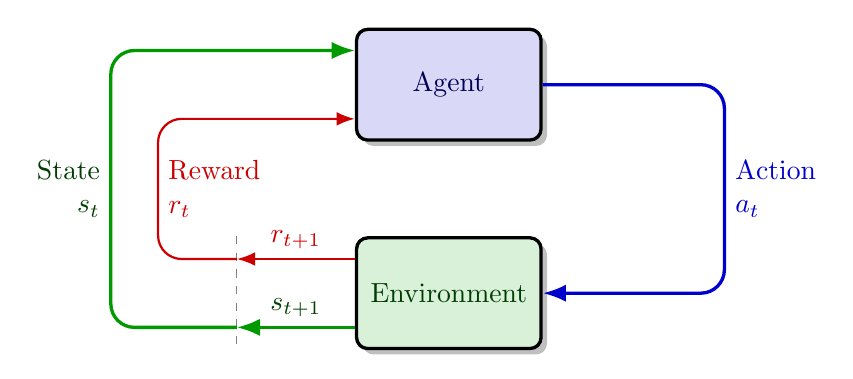
\begin{tikzpicture}[very thick, node distance=4cm]
                            % Colored nodes
                            \node [frame, fill=myblue!15, text=mydarkblue] (agent) {Agent};
                            \node [frame, below=1.2cm of agent, fill=mygreen!15, text=mydarkgreen] (environment) {Environment};
                            % Action (blue)
                            \draw[line, myblue] (agent) -- ++ (3.5,0) |- (environment)
                            node[right, pos=0.25, align=left, text=myblue] {Action\\ $a_t$};
                            % Separator
                            \coordinate[left=15mm of environment] (P);
                            \draw[thin, dashed, gray] (P|-environment.north) -- (P|-environment.south);
                            % State (green)
                            \draw[line, mygreen] (environment.200) -- (P |- environment.200)
                            node[midway, above, text=mydarkgreen] {$s_{t+1}$};
                            \draw[line, mygreen] (P |- environment.200) -- ++ (-1.6,0) |- (agent.160)
                            node[left, pos=0.25, align=right, text=mydarkgreen] {State\\ $s_t$};
                            % Reward (red)
                            \draw[line, thick, myred] (environment.160) -- (P |- environment.160)
                            node[midway, above, text=myred] {$r_{t+1}$};
                            \draw[line, thick, myred] (P |- environment.160) -- ++ (-1,0) |- (agent.200)
                            node[right, pos=0.25, align=left, text=myred] {Reward\\ $r_t$};
                \end{tikzpicture}%
                }
                \caption{\footnotesize Agent-Environment Interaction Loop}
                \label{fig:agent_env_en}
            \end{figure}
        \end{column}
    \end{columns}
\end{frame}

\begin{frame}
    \frametitle{State, Observations, and Actions}
    \begin{itemize}
        \item \textbf{State ($\boldsymbol{s}$):} Complete description of the environment at a given time
        \begin{itemize}\setlength{\itemsep}{4pt}
            \item Encodes all variables needed to predict future dynamics
            \item Typically hidden from the agent in real-world problems
        \end{itemize}
        
        \item \textbf{Observation ($\boldsymbol{o}$):} Information perceived by the agent
        \begin{itemize}\setlength{\itemsep}{4pt}
            \item May be noisy or incomplete (partial observability)
            \item In fully observable environments: $s = o$
            \item In partially observable settings: agent must infer hidden aspects of $s$
        \end{itemize}
        
        \item \textbf{Action Space ($\mathcal{A}$):} Set of all possible actions an agent can take
        \begin{itemize}\setlength{\itemsep}{4pt}
            \item \textbf{Discrete:} Finite set of actions (e.g., \texttt{up, down, left, right})
            \item \textbf{Continuous:} Actions represented by real values (e.g., steering angle, force applied)
            % \item Can be multi-dimensional, combining discrete and continuous aspects
        \end{itemize}
    \end{itemize}
\end{frame}



\begin{frame}
    \frametitle{Trajectory and Reward}
    \begin{columns}[T]
        \begin{column}{0.5\textwidth}
            \textbf{Definitions:}
            \begin{itemize}\setlength{\itemsep}{6pt}
                \item Trajectory: sequence of states and actions the agent experiences over time.
                \item Reward: scalar feedback provided by the environment after taking an action.
                \item Return: accumulated reward over a trajectory (finite or discounted horizon).
            \end{itemize}
        \end{column}
        
        \begin{column}{0.5\textwidth}
            \textbf{Equations:}
            \begin{align*}
                \tau &= (s_0, a_0, s_1, a_1, \ldots) \\
                r_t &= R(s_t, a_t, s_{t+1}) \quad \text{or} \quad r_t = R(s_t, a_t) \\
                R(\tau) &= r_1 + r_2 + \cdots + r_T =
                \sum_{t = 0}^{T} r_t ~ \text{\footnotesize(finite horizon)} \\
                R(\tau) &= r_1 + \gamma r_2 + \gamma^2 r_3 + \cdots =
                \sum_{t = 0}^{\infty} \gamma^t r_t ~ \text{\footnotesize (discounted)}
            \end{align*}
        \end{column}
    \end{columns}
\end{frame}




\begin{frame}
    \frametitle{Policy}
    \begin{itemize}
        \item \textbf{Policy:} Rules that an agent uses to decide which actions to take
    \end{itemize}
    \vspace{5pt}
    \begin{columns}[T]
        \begin{column}{0.55\textwidth}
            \begin{itemize}
                \item \textbf{Types:}
                \begin{itemize}\itemsep=2pt 
                    \item \textbf{Deterministic:} $a_t = \mu(s_t)\to \text{DDPG, TD3}
                    $
                    \item \textbf{Stochastic:} $a_t \sim \pi(\cdot | s_t)\to \text{PPO, SAC}
                    $
                \end{itemize}
                \item \textbf{Parameterized Policy:} Output is a function of policy parameters (neural network weights)
                \begin{itemize}\itemsep=2pt 
                    \item $a_t = \mu_{\theta}(s_t)$ or $a_t \sim \pi_{\theta}(\cdot | s_t)$
                    \item Parameters $\theta$ are optimized during learning
                \end{itemize}
            \end{itemize}
        \end{column}
        
        \begin{column}{0.35\textwidth}
            \vspace{-1cm}
            \begin{figure}
                \captionsetup[subfloat]{labelfont={color=blue,tiny},textfont=footnotesize,skip=20pt}
                \centering
                \resizebox{.9\textwidth}{!}{%
                \begin{tikzpicture}[x=2.4cm,y=1.2cm]
		\readlist\Nnod{4,5,5,2} % array of number of nodes per layer
		\readlist\Nstr{n,32,k} % array of string number of nodes per layer
		\readlist\Cstr{x,h^{(\prev)},u} % array of coefficient symbol per layer
		\def\yshift{0.55} % shift last node for dots
		% LOOP over LAYERS
		\foreachitem \N \in \Nnod{
			\def\lay{\Ncnt} % alias of index of current layer
			\pgfmathsetmacro\prev{int(\Ncnt-1)} % number of previous layer
			\foreach \i [evaluate={\c=int(\i==\N);
				\layercheck=\ifnum\Ncnt=1 0 \else \ifnum\Ncnt=\Nnodlen 0 \else \yshift \fi \fi;
				\y=\N/2-\i*1.2-\c*\layercheck;
				\x=\lay; \n=\nstyle;
				\index=(\i<\N?int(\i):"\Nstr[\n]");}] in {1,...,\N}{ % loop over nodes
				% NODES
				\ifnum \lay=1
				\ifnum \i=1
				\node[node \n] (N\lay-\i) at (\x,\y) {$\delta x$};
				\fi
				\ifnum \i=2
				\node[node \n] (N\lay-\i) at (\x,\y) {$\delta y$};
				\fi
				\ifnum \i=3
				\node[node \n] (N\lay-\i) at (\x,\y) {$\delta {\dot{x}}$};
				\fi
				\ifnum \i=4
				\node[node \n] (N\lay-\i) at (\x,\y) {$\delta {\dot{y}}$};
				\fi
				\else \ifnum \lay=\Nnodlen
				\ifnum \i=1
				\node[node \n] (N\lay-\i) at (\x,\y) {$u_x$};
				\fi
				\ifnum \i=2
				\node[node \n] (N\lay-\i) at (\x,\y) {$u_y$};
				\fi
				\else
				\node[node \n] (N\lay-\i) at (\x,\y) {$\strut\Cstr[\n]_{\index}$};
				\fi \fi
				% CONNECTIONS
				\ifnumcomp{\lay}{>}{1}{ % connect to previous layer
					\foreach \j in {1,...,\Nnod[\prev]}{ % loop over nodes in previous layer
						\draw[white,line width=1.2,shorten >=1] (N\prev-\j) -- (N\lay-\i);
						\draw[connect] (N\prev-\j) -- (N\lay-\i);
					}
				}{}
			}
			% Dots (skip first and last layers)
			\ifnum \lay>1 \ifnum \lay<\Nnodlen
			\path (N\lay-\N) --++ (0,1+\yshift) node[midway,scale=1.6] {$\vdots$}; % dots
			\fi \fi
		}
		% LABELS
		\node[above=.1,align=center,mydarkgreen] at (N1-1.90) {Input\\[-0.2em]Layer};
		\node[above=.1,align=center,mydarkblue] at (N2-1.90) {Hidden\\[-0.2em]Layer};
		\node[above=.1,align=center,mydarkblue] at (N3-1.90) {Hidden\\[-0.2em]Layer};
		\node[above=.1,align=center,mydarkred] at (N\Nnodlen-1.90) {Output\\[-0.2em]Layer};
	\end{tikzpicture}%
                }
                \captionsetup{labelfont={color=myBlue,scriptsize},textfont=scriptsize,skip=8pt}
                \caption{Policy Neural Network Structure}
                \label{fig:actor_nn_en}
            \end{figure}
        \end{column}
    \end{columns}
\end{frame}



\begin{frame}
    \frametitle{Value and Action-Value Functions}
    \begin{itemize}
        \item \textbf{Value Function:} Expected return when following a policy
    \end{itemize}
    \vspace{5pt}
    \setlength{\itemsep}{6pt}
    \begin{columns}[T]
        \begin{column}{0.55\textwidth}
            \textbf{Value Function:}
            \begin{align*}
                V^{\pi}(s) &= \underset{\tau \sim \pi}{\mathbb{E}}\left[R(\tau)|s_0 = s\right]
            \end{align*}
            \vspace{0.3cm}
            \textbf{Action-Value Function:}
            \begin{align*}
                Q^{\pi}(s,a) &= \underset{\tau \sim \pi}{\mathbb{E}}\left[R(\tau)|s_0 = s, a_0 = a\right]
            \end{align*}
            \vspace{0.3cm}
            \textbf{Advantage Function:}
            \begin{align*}
                A^{\pi}(s,a) = Q^{\pi}(s,a) - V^{\pi}(s)
            \end{align*}
        \end{column}
        
        \begin{column}{0.35\textwidth}
            \vspace{-1.1cm}
            % \hspace{.9cm}
            \begin{figure}
                % \centering
                \resizebox{.90\textwidth}{!}{%
                \begin{tikzpicture}[x=2.8cm,y=1.5cm]
                    \readlist\Nnod{6,7,7,1} % array of number of nodes per layer
                    \readlist\Nstr{n,32,k} % array of string number of nodes per layer
                    \readlist\Cstr{x,h^{(\prev)},u} % array of coefficient symbol per layer
                    \def\yshift{0.55} % shift last node for dots
                    
                    % LOOP over LAYERS
                    \foreachitem \N \in \Nnod{
                        \def\lay{\Ncnt} % alias of index of current layer
                        \pgfmathsetmacro\prev{int(\Ncnt-1)} % number of previous layer
                        \foreach \i [evaluate={\c=int(\i==\N); 
                            \layercheck=\ifnum\Ncnt=1 0 \else \ifnum\Ncnt=\Nnodlen 0 \else \yshift \fi \fi;
                            \y=\N/2-\i-\c*\layercheck;
                            \x=\lay; \n=\nstyle;
                            \index=(\i<\N?int(\i):"\Nstr[\n]");}] in {1,...,\N}{ % loop over nodes
                            % NODES
                            \ifnum \lay=1
                            \ifnum \i=1
                            \node[node \n] (N\lay-\i) at (\x,\y) {$\delta x$};
                            \fi
                            \ifnum \i=2
                            \node[node \n] (N\lay-\i) at (\x,\y) {$\delta y$};
                            \fi
                            \ifnum \i=3
                            \node[node \n] (N\lay-\i) at (\x,\y) {$\delta {\dot{x}}$};
                            \fi
                            \ifnum \i=4
                            \node[node \n] (N\lay-\i) at (\x,\y) {$\delta {\dot{y}}$};
                            \fi
                            \ifnum \i=5
                            \node[node \n] (N\lay-\i) at (\x,\y) {$u_x$};
                            \fi
                            \ifnum \i=6
                            \node[node \n] (N\lay-\i) at (\x,\y) {$u_y$};
                            \fi
                            \else \ifnum \lay=\Nnodlen
                            \ifnum \i=1
                            \node[node \n] (N\lay-\i) at (\x,\y) {$Q$};
                            \fi
                            \ifnum \i=2
                            \node[node \n] (N\lay-\i) at (\x,\y) {$u_y$};
                            \fi
                            \else
                            \node[node \n] (N\lay-\i) at (\x,\y) {$\strut\Cstr[\n]_{\index}$};
                            \fi \fi
                            % CONNECTIONS
                            \ifnumcomp{\lay}{>}{1}{ % connect to previous layer
                                \foreach \j in {1,...,\Nnod[\prev]}{ % loop over nodes in previous layer
                                    \draw[white,line width=1.2,shorten >=1] (N\prev-\j) -- (N\lay-\i);
                                    \draw[connect] (N\prev-\j) -- (N\lay-\i);
                                }
                            }{}
                        }
                        
                        % Dots (skip first and last layers)
                        \ifnum \lay>1 \ifnum \lay<\Nnodlen
                        \path (N\lay-\N) --++ (0,1+\yshift) node[midway,scale=1.6] {$\vdots$}; % dots
                        \fi \fi
                    }
                    
                    % LABELS
                    \node[above=.1,align=center,mydarkgreen] at (N1-1.90) {Input\\[-0.2em]Layer};
                    \node[above=.1,align=center,mydarkblue] at (N2-1.90) {Hidden\\[-0.2em]Layer};
                    \node[above=.1,align=center,mydarkblue] at (N3-1.90) {Hidden\\[-0.2em]Layer};
                    \node[above=.1,align=center,mydarkred] at (N\Nnodlen-1.25) {Output\\[-0.2em]Layer};
                \end{tikzpicture}
                }
                \captionsetup{labelfont={color=myBlue,scriptsize},textfont=scriptsize,skip=4pt}
                \caption{Action-Value Function Neural Network}
                \label{fig:critic_nn_en}
            \end{figure}
        \end{column}
    \end{columns}
\end{frame}

% \begin{frame}
%     \frametitle{Optimal Value Functions}
    
%     \begin{columns}[T]
%         \begin{column}{0.5\textwidth}
%             \textbf{Optimal State Value Function:}
%             \begin{align*}
%                 V^{*}(s) &= \underset{\pi}{\max} V^{\pi}(s)
%             \end{align*}
%             \vspace{0.1cm}
%             \textbf{Optimal Value Bellman Equation:}
%             \begin{align*}
%                 V^{*}(s) &= \max_a \underset{s'\sim P}{\mathrm{E}} \left[ r(s,a) + \gamma V^{*}(s') \right]
%             \end{align*}
%         \end{column}
        
%         \begin{column}{0.5\textwidth}
%             \textbf{Optimal Action-Value Function:}
%             \begin{align*}
%                 Q^{*}(s,a) &= \underset{\pi}{\max} Q^{\pi}(s,a)
%             \end{align*}
%             \vspace{0.1cm}
%             \textbf{Optimal Q Bellman Equation:}
%             \begin{align*}
%                 Q^{*}(s,a) &= r(s,a) + \gamma \underset{s'\sim P}{\mathrm{E}} \left[ \max_{a'} Q^{*}(s',a') \right]
%             \end{align*}
%         \end{column}
%     \end{columns}
    
%     % \vspace{0.4cm}
%     \begin{minipage}{0.83\textwidth}
%     \begin{block}{Value Computation}
%         How can we calculate the value of a state $V(s)$ 
%         and a state-action pair $Q(s,a)$?
%     \end{block}
% \end{minipage}

% \end{frame}

% \begin{frame}
%     \frametitle{Bellman Equations}
    
%     \textbf{For Policy Value Functions:}
%     \begin{align*}
%         V^{\pi}(s) &= \underset{\substack{a \sim \pi \\ s'\sim P}}{\mathrm{E}} 
%         \left[ r(s,a) + \gamma V^{\pi}(s') \right] \\
%         Q^{\pi}(s,a) &= r(s,a) + \gamma \underset{s'\sim P}{\mathrm{E}} 
%         \left[ \underset{a'\sim \pi}{\mathrm{E}} \left[ Q^{\pi}(s',a') \right] \right]
%     \end{align*}
    
%     \vspace{0.3cm}
%     \textbf{For Optimal Value Functions:}
%     \begin{align*}
%         V^{*}(s) &= \max_a \underset{s'\sim P}{\mathrm{E}} \left[ r(s,a) + \gamma V^{*}(s') \right] \\
%         Q^{*}(s,a) &= r(s,a) + \gamma \underset{s'\sim P}{\mathrm{E}} \left[ \max_{a'} Q^{*}(s',a') \right]
%     \end{align*}
% \end{frame}



\begin{frame}
  \frametitle{Value Computation and Bellman Equations}

  \begin{block}{Value Computation}
    How can we calculate the value of a state $V(s)$ 
    and a state-action pair $Q(s,a)$?
  \end{block}

%   \vspace{0.3cm}

  \textbf{For Policy Value Functions:}
  \begin{align*}
      V^{\pi}(s) &= \underset{\substack{a \sim \pi \\ s'\sim P}}{\mathrm{E}} 
      \left[ r(s,a) + \gamma V^{\pi}(s') \right] \\[-.5em]
      Q^{\pi}(s,a) &= r(s,a) + \gamma \underset{s'\sim P}{\mathrm{E}} 
      \left[ \underset{a'\sim \pi}{\mathrm{E}} \left[ Q^{\pi}(s',a') \right] \right]
  \end{align*}

%   \vspace{0.3cm}

  \textbf{For Optimal Value Functions:}
  \begin{align*}
    V^{*}(s) = \underset{\pi}{\max} V^{\pi}(s) \to
      V^{*}(s) &= \max_a \underset{s'\sim P}{\mathrm{E}} \left[ r(s,a) + \gamma V^{*}(s') \right] \\[-.5em]
      Q^{*}(s,a) = \underset{\pi}{\max} Q^{\pi}(s,a) \to
      Q^{*}(s,a) &= r(s,a) + \gamma \underset{s'\sim P}{\mathrm{E}} \left[ \max_{a'} Q^{*}(s',a') \right]
  \end{align*}

\end{frame}

\section{RL Algorithms}
\begin{frame}
    \frametitle{DDPG Algorithm}
    % \small\begin{algorithm}[H]
        \begin{algorithmic}[1]
    \STATE Initialize: policy $\theta$, Q-function $\phi$, targets $\theta_{\text{targ}}$, $\phi_{\text{targ}}$, replay buffer $\mathcal{D}$
    \REPEAT
        \STATE Collect experience: $a = \text{clip}(\mu_{\theta}(s) + \text{noise})$, observe $(s',r,d)$, store in $\mathcal{D}$
        \STATE Sample batch $B$ from $\mathcal{D}$
        \STATE Compute targets: $y = r + \gamma (1-d) Q_{\phi_{\text{targ}}}(s', \mu_{\theta_{\text{targ}}}(s'))$
        \STATE Update critic: minimize $(Q_{\phi}(s,a) - y)^2$
        \STATE Update actor: maximize $Q_{\phi}(s, \mu_{\theta}(s))$
        \STATE Update targets: $\phi_{\text{targ}} \leftarrow \rho \phi_{\text{targ}} + (1-\rho) \phi$, same for $\theta$
    \UNTIL{convergence}
    \end{algorithmic}
% \end{algorithm}
\end{frame}

\begin{frame}
    \frametitle{Twin Delayed DDPG (TD3) Algorithm}
    \vspace{-0.25cm}
    % \footnotesize\begin{algorithm}[H]
        \begin{algorithmic}[1]
    \STATE Initialize: policy $\theta$, Q-functions $\phi_1$, $\phi_2$, targets $\theta_{\text{targ}}$, $\phi_{\text{targ},1}$, $\phi_{\text{targ},2}$, buffer $\mathcal{D}$
    \REPEAT
        \STATE Collect experience: $a = \text{clip}(\mu_{\theta}(s) + \text{noise}, a_{Low}, a_{High})$
        \STATE Store transition $(s,a,r,s',d)$ in $\mathcal{D}$
        \IF{time to update}
            \STATE Sample batch $B$ from $\mathcal{D}$
            \STATE Compute target actions with noise: $a'(s') = \text{clip}(\mu_{\theta_{\text{targ}}}(s') + \text{noise}, a_{Low}, a_{High})$
            \STATE Compute targets: $y = r + \gamma (1-d) \min_{i=1,2} Q_{\phi_{\text{targ},i}}(s', a'(s'))$
            \STATE Update Q-functions: minimize $(Q_{\phi_i}(s,a) - y)^2$ for $i=1,2$
            % \IF{delay counter $\mod$ \texttt{policy\_delay} $ = 0$}
                \STATE Update policy: maximize $Q_{\phi_1}(s, \mu_{\theta}(s))$
                \STATE Update targets: $\phi_{\text{targ},i} \leftarrow \rho \phi_{\text{targ},i} + (1-\rho) \phi_i$ for $i=1,2$
                \STATE Update target policy: $\theta_{\text{targ}} \leftarrow \rho \theta_{\text{targ}} + (1-\rho) \theta$
            % \ENDIF
        \ENDIF
    \UNTIL{convergence}
    \end{algorithmic}
% \end{algorithm}
\end{frame}

\begin{frame}
    \frametitle{Soft Actor-Critic (SAC) Algorithm}
    \vspace{-0.25cm}
    \begin{algorithmic}[1]
    \STATE Initialize: policy $\theta$, Q-functions $\phi_1$, $\phi_2$, targets $\phi_{\text{targ},1}$, $\phi_{\text{targ},2}$, buffer $\mathcal{D}$
    \REPEAT
        \STATE Collect experience: $a \sim \pi_{\theta}(\cdot|s)$, observe $(s',r,d)$, store in $\mathcal{D}$
        \IF{time to update}
            \STATE Sample batch $B$ from $\mathcal{D}$
            \STATE Sample actions from policy: $\tilde{a}' \sim \pi_{\theta}(\cdot|s')$
            \STATE Compute targets: $y = r + \gamma (1-d) \left(\min_{i=1,2} Q_{\phi_{\text{targ}, i}} (s', \tilde{a}') - \alpha \log \pi_{\theta}(\tilde{a}'|s')\right)$
            \STATE Update Q-functions: minimize $(Q_{\phi_i}(s,a) - y)^2$ for $i=1,2$
            \STATE Sample actions using reparameterization trick: $\tilde{a}_{\theta}(s) \sim \pi_{\theta}(\cdot|s)$
            \STATE Update policy: maximize $\min_{i=1,2} Q_{\phi_i}(s, \tilde{a}_{\theta}(s)) - \alpha \log \pi_{\theta}(\tilde{a}_{\theta}(s)|s)$
            \STATE Update targets: $\phi_{\text{targ},i} \leftarrow \rho \phi_{\text{targ},i} + (1-\rho) \phi_i$ for $i=1,2$
        \ENDIF
    \UNTIL{convergence}
    \end{algorithmic}
\end{frame}

\begin{frame}
    \frametitle{Proximal Policy Optimization (PPO) Algorithm}
    \vspace{-0.25cm}
    \begin{algorithmic}[1]
    \STATE Initialize: policy $\theta_0$, value function $\phi_0$
    \FOR{$k = 0,1,2,...$}
        \STATE Collect trajectories ${\mathcal D}_k = \{\tau_i\}$ by running policy $\pi_k = \pi(\theta_k)$ in environment
        \STATE Compute rewards-to-go $\hat{R}_t$
        \STATE Compute advantage estimates $\hat{A}_t$ based on current value function $V_{\phi_k}$
        \STATE Update policy by maximizing the PPO-Clip objective:
        \begin{align*}
            \theta_{k+1} = \arg \max_{\theta} \frac{1}{|{\mathcal D}_k|} \sum_{\tau, t} \min\left(
                r_t(\theta) \hat{A}_t, \; \text{clip}(r_t(\theta), 1-\epsilon, 1+\epsilon) \hat{A}_t
            \right)
        \end{align*}
        where $r_t(\theta) = \frac{\pi_{\theta}(a_t|s_t)}{\pi_{\theta_k}(a_t|s_t)}$ is the probability ratio
        \STATE Fit value function by minimizing:
        \begin{align*}
            \phi_{k+1} = \arg \min_{\phi} \frac{1}{|{\mathcal D}_k|} \sum_{\tau, t}\left( V_{\phi}(s_t) - \hat{R}_t \right)^2
        \end{align*}
    \ENDFOR
    \end{algorithmic}
\end{frame}
\chapter{یادگیری تقویتی چندعاملی}
کاربردهای پیچیده در یادگیری تقویتی نیازمند اضافه کردن چندین عامل\LTRfootnote{Multi-Agent} برای انجام همزمان وظایف مختلف هستند.
با این حال، افزایش تعداد عامل‌ها چالش‌هایی در مدیریت تعاملات میان آن‌ها به همراه دارد.
در این فصل، بر اساس مسئله بهینه‌سازی برای هر عامل، مفهوم تعادل\LTRfootnote{Equilibrium} معرفی شده تا رفتارهای توزیعی چندعاملی را تنظیم کند.
رابطه رقابت میان عامل‌ها در سناریوهای مختلف تحلیل شده و آن‌ها با الگوریتم‌های معمول یادگیری تقویتی چندعاملی ترکیب شده‌اند. بر اساس انواع تعاملات، یک چارچوب نظریه بازی برای مدل‌سازی عمومی در سناریوهای چندعاملی استفاده شده است. با تحلیل بهینه‌سازی و وضعیت تعادل برای هر بخش از چارچوب، سیاست بهینه یادگیری تقویتی چندعاملی برای هر عامل بررسی شده است. در این فصل ابتدا در بخش \ref{sec:marl_definitions} مفاهیم اولیه یادگیری تقویتی چندعاملی معرفی شده است.
 سپس در بخش \ref{sec:marl_games} انواع بازی‌ها و تعادل نش مورد بررسی قرار گرفته است.
الگوریتم‌های مختلف یادگیری تقویتی چندعاملی شامل
 \lr{MA-DDPG}
 در بخش
  \ref{sec:marl_maddpg}،
   \lr{MA-TD3}
    در بخش \ref{sec:MATD3}،
    \lr{MA-SAC} در بخش \ref{sec:MASAC} و \lr{MA-PPO} در بخش \ref{sec:MAPPO} معرفی و بررسی شده‌اند.
  \section{تعاریف و مفاهیم اساسی }\label{sec:marl_definitions}
یادگیری تقویتی چندعاملی\LTRfootnote{Multi-Agent Reinforcement Learning (MARL)} به بررسی چگونگی یادگیری و تصمیم‌گیری چندین عامل مستقل در یک محیط مشترک پرداخته می‌شود. برای تحلیل دقیق و درک بهتر این حوزه، اجزای اصلی آن شامل عامل، سیاست و مطلوبیت\LTRfootnote{Utility} در نظر گرفته می‌شوند که در ادامه به صورت مختصر و منسجم تشریح می‌گردند.

\begin{itemize}
	\item عامل: یک موجودیت مستقل به عنوان عامل تعریف می‌شود که به صورت خودمختار با محیط تعامل کرده و بر اساس مشاهدات رفتار سایر عامل‌ها، سیاست‌هایش انتخاب می‌گردند تا سود حداکثر یا ضرر حداقل حاصل شود. در سناریوهای مورد بررسی، چندین عامل به صورت مستقل عمل می‌کنند؛ اما اگر تعداد عامل‌ها به یک کاهش یابد، \lr{MARL} به یادگیری تقویتی معمولی تبدیل می‌شود.
	
	\item سیاست: برای هر عامل در \lr{MARL}، سیاستی خاص در نظر گرفته می‌شود که به عنوان روشی برای انتخاب اقدامات بر اساس وضعیت محیط و رفتار سایر عامل‌ها تعریف می‌گردد. این سیاست‌ها با هدف به حداکثر رساندن سود و به حداقل رساندن هزینه طراحی شده و تحت تأثیر محیط و سیاست‌های دیگر عامل‌ها قرار می‌گیرند.
	
	\item مطلوبیت: مطلوبیت
	هر عامل بر اساس نیازها و وابستگی‌هایش به محیط و سایر عامل‌ها تعریف شده و به صورت سود منهای هزینه، با توجه به اهداف مختلف محاسبه می‌شود. در سناریوهای چندعاملی، از طریق یادگیری از محیط و تعامل با دیگران، مطلوبیت هر عامل بهینه می‌گردد.
\end{itemize}

در این چارچوب، برای هر عامل در \lr{MARL} تابع مطلوبیت خاصی در نظر گرفته شده و بر اساس مشاهدات و تجربیات حاصل از تعاملات، یادگیری سیاست به صورت مستقل انجام می‌شود تا ارزش مطلوبیت به حداکثر برسد، بدون اینکه مستقیماً به مطلوبیت سایر عامل‌ها توجه شود. این فرآیند ممکن است به رقابت یا همکاری میان عامل‌ها منجر گردد.
 با توجه به پیچیدگی تعاملات میان چندین عامل، تحلیل نظریه بازی‌ها به عنوان ابزاری مؤثر برای تصمیم‌گیری در این حوزه به کار گرفته می‌شود. بسته به سناریوهای مختلف، این بازی‌ها در دسته‌بندی‌های متفاوتی قرار داده شده که در بخش‌های بعدی بررسی خواهند شد.
 
 
 
% \begin{figure}[H]
% 	\begin{center}
% 		\lr{		\begin{tikzpicture}[very thick,node distance = 4cm]
% 				\node [frame] (agent) {Agent};
% 				\node [frame, below=1.2cm of agent] (environment) {Environment};
% 				\draw[line] (agent) -- ++ (3.5,0) |- (environment) 
% 				node[right,pos=0.25,align=left] {action\\ $a_t$};
% 				\coordinate[left=15mm of environment] (P);
% 				\draw[thin,dashed] (P|-environment.north) -- (P|-environment.south);
% 				\draw[line] (environment.200) -- (P |- environment.200)
% 				node[midway,above]{$s_{t+1}$};
% 				\draw[line,thick] (environment.160) -- (P |- environment.160)
% 				node[midway,above]{$r_{t+1}$};
% 				\draw[line] (P |- environment.200) -- ++ (-1.6,0) |- (agent.160)
% 				node[left, pos=0.25, align=right] {state\\ $s_t$};
% 				\draw[line,thick] (P |- environment.160) -- ++ (-1,0) |- (agent.200)
% 				node[right,pos=0.25,align=left] {reward\\ $r_t$};
% 		\end{tikzpicture}}
% 	\end{center}
% 	\caption{حلقه تعامل عامل و محیط}
% 	\label{fig:multi-agent_env}
% \end{figure}
% 
% 
%
% 
% 
%   \begin{figure}[H]
% 	\centering
% 	\lr{\begin{tikzpicture}[very thick, node distance=4cm]
% 		% Define nodes
% 		\node [frame, minimum height=2em] (agent1) {Agent I};
% 		\node [frame, below=1.2cm of agent1, minimum height=6em] (environment) {Environment};
% 		\node [frame, below=1.2cm of environment,minimum height=2em] (agent2) {Agent II};
% 		% Define coordinate for state/reward lines
% 		\coordinate[left=15mm of environment] (P);
% 		% Dashed line separator
% 		\draw[thick, dashed] (P |- environment.north) -- (P |- environment.south);
% 		% Agent I connections
% 		\draw[line] (agent1) -- ++(3.5,0) |- (environment.10) 
% 		node[right, pos=0.25, align=left] {action I\\ $a_1(t)$};
% 		\draw[line] (environment.180) -- (P |- environment.180)
% 		node[midway, above] {\small$s(t+1)$};
% 		\draw[line, thick] (environment.155) -- (P |- environment.155)
% 		node[midway, above] {\small$r_1(t+1)$};
% 		\draw[line] (P |- environment.180) -- ++(-1.6,0) |- (agent1.170)
% 		node[left, pos=0.25, align=right] {state\\ $s(t)$};
% 		\draw[line, thick] (P |- environment.155) -- ++(-1,0) |- (agent1.190)
% 		node[right, pos=0.25, align=left] {reward I\\ $r_1(t)$};
% 		% Agent II connections
% 		\draw[line] (agent2) -- ++(3.5,0) |- (environment.350) 
% 		node[right, pos=0.25, align=left] {action II\\ $a_2(t)$};
% 		\draw[line, thick] (environment.205) -- (P |- environment.205)
% 		node[midway, above] {\small$r_2(t+1)$};
% 		\draw[line] (P |- environment.180) -- ++(-1.6,0) |- (agent2.190)
% 		node[left, pos=0.25, align=right] {state\\ $s(t)$};
% 		\draw[line, thick] (P |- environment.205) -- ++(-1,0) |- (agent2.170)
% 		node[right, pos=0.25, align=left] {reward II\\ $r_2(t)$};
% 	\end{tikzpicture}}
% 	 \caption{حلقه تعامل عامل‌های  یادگیری تقویتی چند عاملی با محیط}
% \end{figure}
% 
% 
% 
% 
% 
% 
% \begin{figure}[H]
% 	\centering
% 	\lr{\begin{tikzpicture}[very thick, node distance=4cm]
% 		% Define nodes with colors
% 		\node [frame, minimum height=2em, fill=myblue!15, text=mydarkblue] (agent1) {Agent I};
% 		\node [frame, below=1.2cm of agent1, minimum height=6em, fill=mygreen!15, text=mydarkgreen] (environment) {Environment};
% 		\node [frame, below=1.2cm of environment, minimum height=2em, fill=myviolet!15, text=myviolet] (agent2) {Agent II}; 		
% 		% Define coordinate for state/reward lines
% 		\coordinate[left=18mm of environment] (P);
% 		% Dashed line separator
% 		\draw[thick, dashed] ($(P|-environment.north)+(0,-3mm)$) -- ($(P|-environment.south)+(0,3.8mm)$);
% 		% Agent I connections - colorized
% 		\draw[line, myblue] (agent1) -- ++(3.5,0) |- (environment.10) 
% 		node[right, pos=0.25, align=left, text=myblue] {action I\\ $a_1(t)$};
% 		\draw[line, mygreen] (environment.180) -- (P |- environment.180)
% 		node[midway, above, text=mydarkgreen] {$s(t+1)$};
% 		\draw[line, thick, myred] (environment.155) -- (P |- environment.155)
% 		node[midway, above, text=myred] {$r_1(t+1)$};
% 		\draw[line, mygreen] (P |- environment.180) -- ++(-1.6,0) |- (agent1.170)
% 		node[left, pos=0.25, align=right, text=mydarkgreen] {state\\ $s(t)$};
% 		\draw[line, thick, myred] (P |- environment.155) -- ++(-1,0) |- (agent1.190)
% 		node[right, pos=0.25, align=left, text=myred] {reward I\\ $r_1(t)$};
% 		% Agent II connections - colorized
% 		\draw[line, myviolet] (agent2) -- ++(3.5,0) |- (environment.350) 
% 		node[right, pos=0.25, align=left, text=myviolet] {action II\\ $a_2(t)$};
% 		\draw[line, thick, myorange] (environment.205) -- (P |- environment.205)
% 		node[midway, above, text=myorange] {$r_2(t+1)$};
% 		\draw[line, mygreen] (P |- environment.180) -- ++(-1.6,0) |- (agent2.190)
% 		node[left, pos=0.25, align=right, text=mydarkgreen] {state\\ $s(t)$};
% 		\draw[line, thick, myorange] (P |- environment.205) -- ++(-1,0) |- (agent2.170)
% 		node[right, pos=0.25, align=left, text=myorange] {reward II\\ $r_2(t)$};
% 	\end{tikzpicture}}
% 	 \caption{حلقه تعامل عامل‌های  یادگیری تقویتی چند عاملی با محیط}
% \end{figure}
 
 
 
 \vspace{10mm}
 
  \begin{figure}[H]
 	\centering
 	\begin{tikzpicture}[very thick, node distance=4cm]
 			% Define nodes with colors
 			\node [frame, minimum height=2em, fill=myblue!15, text=mydarkblue] (agent1) {۱ عامل};
 			\node [frame, below=1.2cm of agent1, minimum height=6em, fill=mygreen!15, text=mydarkgreen] (environment) {محیط};
 			\node [frame, below=1.2cm of environment, minimum height=2em, fill=myviolet!15, text=myviolet] (agent2) {۲ عامل}; 		
 			% Define coordinate for state/reward lines
 			\coordinate[left=18mm of environment] (P);
 			% Dashed line separator
 			\draw[thick, dashed] ($(P|-environment.north)+(0,-3mm)$) -- ($(P|-environment.south)+(0,3.8mm)$);
 			% Agent I connections - colorized
 			\draw[line, myblue] (agent1) -- ++(3.5,0) |- (environment.10) 
 			node[right, pos=0.25, align=left, text=myblue] {۱ عمل\\ $a_1(t)$};
 			\draw[line, mygreen] (environment.180) -- (P |- environment.180)
 			node[midway, above, text=mydarkgreen] {$s(t+1)$};
 			\draw[line, thick, myred] (environment.155) -- (P |- environment.155)
 			node[midway, above, text=myred] {$r_1(t+1)$};
 			\draw[line, mygreen] (P |- environment.180) -- ++(-1.6,0) |- (agent1.170)
 			node[left, pos=0.25, align=right, text=mydarkgreen] {وضعیت\\ $s(t)$};
 			\draw[line, thick, myred] (P |- environment.155) -- ++(-1,0) |- (agent1.190)
 			node[right, pos=0.25, align=left, text=myred] {۱ پاداش\\ $r_1(t)$};
 			% Agent II connections - colorized
 			\draw[line, myviolet] (agent2) -- ++(3.5,0) |- (environment.350) 
 			node[right, pos=0.25, align=left, text=myviolet] {۲ عمل\\ $a_2(t)$};
 			\draw[line, thick, myorange] (environment.205) -- (P |- environment.205)
 			node[midway, above, text=myorange] {$r_2(t+1)$};
 			\draw[line, mygreen] (P |- environment.180) -- ++(-1.6,0) |- (agent2.190)
 			node[left, pos=0.25, align=right, text=mydarkgreen] {وضعیت\\ $s(t)$};
 			\draw[line, thick, myorange] (P |- environment.205) -- ++(-1,0) |- (agent2.170)
 			node[right, pos=0.25, align=left, text=myorange] {۲ پاداش\\ $r_2(t)$};
 	\end{tikzpicture}
 	 \caption{حلقه تعامل عامل‌های  یادگیری تقویتی چند عاملی با محیط}
 \end{figure}

  % \section{اهمیت یادگیری تقویتی چندعاملی}

یادگیری تقویتی چندعاملی به دلیل قابلیت‌های بالقوه‌اش در مدل‌سازی و حل مسائل پیچیده و پویا، اهمیت زیادی در حوزه‌های مختلف علمی و صنعتی دارد. در این بخش، به بررسی اهمیت \lr{MARL} در زمینه‌های مختلف پرداخته و نقش آن را در توسعه سیستم‌های هوشمند متعدد بررسی می‌کنیم.

\subsubsection{مدل‌سازی سیستم‌های پیچیده و پویا}
یکی از دلایل اصلی اهمیت \lr{MARL}، توانایی آن در مدل‌سازی سیستم‌های پیچیده و پویا است. در بسیاری از کاربردهای واقعی، سیستم‌ها شامل چندین عامل هستند که به صورت همزمان و مستقل به تعامل می‌پردازند. به عنوان مثال، در شبکه‌های ترافیکی، هر خودرو می‌تواند به عنوان یک عامل مستقل عمل کند که نیاز به هماهنگی و تعامل با سایر خودروها برای بهینه‌سازی جریان ترافیک دارد. \lr{MARL} با فراهم کردن چارچوبی برای تعامل و یادگیری میان این عوامل، امکان بهبود کارایی و کاهش ترافیک را فراهم می‌کند.

\subsubsection{کاربرد در رباتیک چندعاملی}
در حوزه رباتیک، سیستم‌های چندعاملی می‌توانند برای انجام وظایف پیچیده‌ای مانند جست‌وجو و نجات، حمل و نقل مواد، و عملیات هماهنگ در محیط‌های غیرقابل پیش‌بینی مورد استفاده قرار گیرند. به عنوان مثال، گروهی از ربات‌های پرنده (دُرون‌ها) می‌توانند با همکاری و تبادل اطلاعات، منطقه‌ای وسیع را برای شناسایی اهداف نظارت کنند یا به سرعت به تغییرات محیطی واکنش نشان دهند. \lr{MARL} در این زمینه بهبود هماهنگی میان ربات‌ها و افزایش کارایی عملیات‌های چندعاملی را ممکن می‌سازد.

\subsubsection{مدیریت منابع در شبکه‌های ارتباطی}
شبکه‌های ارتباطی مدرن نیازمند مدیریت بهینه منابع مانند پهنای باند، انرژی و ظرفیت ذخیره‌سازی هستند. در این راستا، \lr{MARL} می‌تواند به عنوان یک ابزار قدرتمند برای تخصیص بهینه منابع به عوامل مختلف شبکه عمل کند. به عنوان مثال، در شبکه‌های بی‌سیم، هر دستگاه کاربر می‌تواند به عنوان یک عامل مستقل عمل کرده و با یادگیری و تعامل با سایر دستگاه‌ها، نحوه بهینه‌سازی مصرف انرژی و پهنای باند را پیدا کند. این امر منجر به افزایش کارایی شبکه و کاهش هزینه‌های عملیاتی می‌شود.

\subsubsection{توسعه الگوریتم‌های پیشرفته‌تر و قابل اعتمادتر}
یکی دیگر از جنبه‌های مهم \lr{MARL}، فهم و تحلیل تعاملات میان عوامل مختلف است که می‌تواند به توسعه الگوریتم‌های پیشرفته‌تر و قابل اعتمادتر منجر شود. با مطالعه رفتارها و استراتژی‌های مختلف در محیط‌های چندعاملی، پژوهشگران قادر به طراحی الگوریتم‌هایی می‌شوند که نه تنها بهینه عمل می‌کنند بلکه مقاومت بالایی در برابر تغییرات محیطی و رفتارهای غیرمنتظره دارند. این الگوریتم‌ها می‌توانند در شرایط متنوع و پیچیده‌تر به خوبی عمل کنند و از خطاها و ناهنجاری‌های احتمالی جلوگیری نمایند.

\subsubsection{کاربرد در بازی‌های چندعاملی و شبیه‌سازی‌های اقتصادی}
بازی‌های چندعاملی و شبیه‌سازی‌های اقتصادی از دیگر حوزه‌هایی هستند که به شدت از \lr{MARL} بهره‌مند می‌شوند. در بازی‌های استراتژیک چند نفره، \lr{MARL} می‌تواند به بازیگران کمک کند تا استراتژی‌های بهینه‌ای برای رقابت و همکاری با یکدیگر توسعه دهند. همچنین، در شبیه‌سازی‌های اقتصادی، \lr{MARL} می‌تواند به مدل‌سازی و تحلیل رفتارهای بازار و تصمیم‌گیری‌های اقتصادی کمک کند، که این امر به پیش‌بینی دقیق‌تر روندهای اقتصادی و بهبود سیاست‌گذاری‌های مالی منجر می‌شود.

\subsubsection{افزایش قابلیت انعطاف‌پذیری و مقیاس‌پذیری سیستم‌ها}
سیستم‌های چندعاملی معمولاً نیازمند قابلیت انعطاف‌پذیری و مقیاس‌پذیری بالا هستند تا بتوانند با تغییرات محیطی و افزایش تعداد عوامل سازگار شوند. \lr{MARL} با استفاده از الگوریتم‌های توزیع‌شده و یادگیری محلی، امکان توسعه سیستم‌هایی با مقیاس بزرگ و پیچیدگی بالا را فراهم می‌کند. این امر به ویژه در کاربردهایی مانند اینترنت اشیاء\LTRfootnote{Internet of Things (IoT)}، هوش مصنوعی توزیع‌شده و سیستم‌های بزرگ‌مقیاس داده‌های بزرگ\LTRfootnote{Big Data}
 بسیار حائز اهمیت است.

%\subsubsection{نتیجه‌گیری}
%در نهایت، یادگیری تقویتی چندعاملی به عنوان یک ابزار قدرتمند در حل مسائل پیچیده و پویا مطرح است که قابلیت‌های متنوعی در حوزه‌های مختلف علمی و صنعتی ارائه می‌دهد. از مدل‌سازی سیستم‌های پیچیده و رباتیک چندعاملی گرفته تا مدیریت منابع در شبکه‌های ارتباطی و توسعه الگوریتم‌های پیشرفته‌تر، \lr{MARL} نقش کلیدی در پیشرفت تکنولوژی‌های هوشمند و خودکار ایفا می‌کند. با ادامه تحقیقات و بهبود الگوریتم‌های موجود، انتظار می‌رود که کاربردهای \lr{MARL} همچنان گسترش یافته و تاثیرات مثبتی در حوزه‌های مختلف داشته باشد.


    \subsection{بازی‌های جمع صفر}

بازی‌های جمع صفر\LTRfootnote{Zero-Sum}
 یکی از انواع اصلی بازی‌های چندعاملی هستند که در آن سود یک بازیکن به طور مستقیم با ضرر بازیکنان دیگر مرتبط است. در این بازی‌ها، مجموع پاداش‌ها برای همه بازیکنان در هر حالت برابر با صفر است، به این معنی که هر افزایشی در پاداش یکی از بازیکنان منجر به کاهش معادل آن در بازیکنان دیگر می‌شود. این نوع بازی‌ها به خوبی می‌توانند رقابت‌های شدید و استراتژی‌های بهینه را مدل‌سازی کنند.

بازی‌های جمع صفر می‌توانند بر اساس سناریوهای مختلف به دسته‌های متنوعی تقسیم‌بندی شوند. دو دسته اصلی این بازی‌ها عبارتند از بازی‌های ثابت و بازی‌های تکراری.

\begin{itemize}
	\item \textbf{بازی ثابت (\lr{Static Game}):} بازی ثابت ساده‌ترین شکل برای مدل‌سازی تعاملات میان عوامل است. در بازی ثابت، هر عامل تنها یک تصمیم‌گیری واحد را انجام می‌دهد. از آنجایی که هر عامل تنها یک بار عمل می‌کند، تقلب و خیانت غیرمنتظره می‌تواند در این نوع بازی‌ها سودآور باشد. بنابراین، هر عامل نیاز دارد تا به دقت استراتژی‌های سایر عوامل را پیش‌بینی کند تا بتواند به طور هوشمندانه عمل کرده و بیشترین سود ممکن را کسب کند. بازی‌های ثابت معمولاً در سناریوهای رقابتی با تعاملات کوتاه مدت کاربرد دارند.
	
	\item \textbf{بازی تکراری (\lr{Repeated Game}):} بازی تکراری به وضعیتی اشاره دارد که در آن تمام عوامل می‌توانند بر اساس همان وضعیت برای چندین تکرار اقداماتی انجام دهند. سود کلی هر عامل مجموع سودهای تخفیف‌شده برای هر تکرار از بازی است. به دلیل اقدامات مکرر تمام عوامل، تقلب و خیانت در طول تعاملات می‌تواند منجر به مجازات یا انتقام از سوی سایر عوامل در تکرارهای آینده شود. بنابراین، بازی تکراری از رفتارهای مخرب عوامل جلوگیری می‌کند و به طور کلی سود کل برای تمام عوامل را افزایش می‌دهد. بازی‌های تکراری معمولاً در سناریوهای همکاری بلندمدت و تعاملات پویا کاربرد دارند.
\end{itemize}

این دسته‌بندی‌ها به محققان و توسعه‌دهندگان کمک می‌کنند تا بازی‌های چندعاملی را بر اساس ویژگی‌های مختلف آن‌ها شناسایی و تحلیل کنند. در بازی‌های ثابت، تمرکز بر پیش‌بینی دقیق استراتژی‌های دیگر عوامل و اتخاذ بهترین تصمیم در یک لحظه زمانی است. در مقابل، بازی‌های تکراری نیازمند توسعه استراتژی‌های پایدار و قابل اعتماد هستند که نه تنها در تکرار اول بلکه در تکرارهای بعدی نیز موثر باشند.

بازی‌های جمع صفر در یادگیری تقویتی چندعاملی به دلیل سادگی و قابلیت مدل‌سازی دقیق تعاملات رقابتی، به عنوان یک ابزار قدرتمند برای تحلیل و توسعه الگوریتم‌های \lr{MARL} مورد استفاده قرار می‌گیرند. این بازی‌ها امکان بررسی رفتارهای استراتژیک، بهینه‌سازی سیاست‌ها و تحلیل تعادل‌های نش (\lr{Nash Equilibrium}) را فراهم می‌کنند که در نهایت به بهبود عملکرد سیستم‌های چندعاملی منجر می‌شود.

\paragraph{مثال‌ها و کاربردها}
یکی از مثال‌های معروف بازی‌های جمع صفر، بازی شطرنج است که در آن هر حرکت یک بازیکن مستقیماً به نفع یا ضرر بازیکن دیگر است. سایر مثال‌ها شامل بازی‌های استراتژیک مانند \lr{Poker} و \lr{Go} می‌باشند که در آن‌ها تعاملات رقابتی میان بازیکنان به طور کامل با اصول بازی‌های جمع صفر مطابقت دارند.

در حوزه‌های عملی، بازی‌های جمع صفر می‌توانند برای مدل‌سازی رقابت‌های بازار، مذاکرات اقتصادی و حتی تعاملات میان ربات‌های خودران در محیط‌های رقابتی مورد استفاده قرار گیرند. این کاربردها به محققان امکان می‌دهند تا الگوریتم‌هایی طراحی کنند که قادر به بهینه‌سازی عملکرد در شرایط رقابتی و متغیر باشند.

\paragraph{چالش‌ها و فرصت‌ها}
یکی از چالش‌های اصلی در بازی‌های جمع صفر، پیش‌بینی دقیق رفتارهای رقبا و اتخاذ تصمیم‌های بهینه در مواجهه با استراتژی‌های متغیر آن‌ها است. همچنین، در بازی‌های تکراری، ایجاد تعادل‌های پایدار و جلوگیری از رفتارهای مخرب به عنوان یک چالش مهم مطرح است. با این حال، این چالش‌ها فرصت‌های قابل توجهی برای توسعه الگوریتم‌های پیشرفته و افزایش قابلیت‌های یادگیری تقویتی چندعاملی فراهم می‌کنند که می‌توانند در شرایط پیچیده‌تر و پویا نیز عملکرد مطلوبی داشته باشند.

    \subsection{تعادل نش}
تعادل نش\LTRfootnote{Nash Equilibrium}
 یکی از بنیادی‌ترین مفاهیم در نظریه بازی‌ها است که توسط جان نش در سال 1950 معرفی شد. این مفهوم به مجموعه‌ای از ‌بازی‌ها اشاره دارد که در آن هیچ بازیکنی نمی‌تواند با تغییر یک‌جانبه سیاست خود، سود بیشتری به دست آورد، به شرطی که سیاست‌های سایر بازیکنان ثابت بماند.


\begin{itemize}
	\item تعریف تعادل نش:
	فرض کنید یک بازی با \( n \) بازیکن داریم. هر بازیکن \( i \) دارای مجموعه سیاست‌های \( \Pi_i \) و تابع مطلوبیت \( u_i: \Pi_1 \times \Pi_2 \times \cdots \times \Pi_n \rightarrow \mathbb{R} \) است. یک مجموعه سیاست \( \pi^* = (\pi_1^*, \pi_2^*, \ldots, \pi_n^*) \) تعادل نش نامیده می‌شود اگر برای هر بازیکن \( i \) و هر سیاست \( \pi_i \in \Pi_i \)
	 در وضعیت \(s\)
	 داشته باشیم:
\begin{equation}
		u_i(\pi_i^*, \pi_{-i}^*, s) \geq u_i(\pi_i, \pi_{-i}^*, s)
\end{equation}
	
	در اینجا، \( \pi_{-i}^* \) نشان‌دهنده سیاست‌های همه بازیکنان به جز بازیکن \( i \) است. در ادامه پژوهش جهت استفاده از چارچوب نظریه بازی در یادگیری تقویتی تابع مطلوبیت به‌گونه‌ای تعریف شده است که برابر با تابع ارزش
	\(u_i(\pi_i, \pi_{-i}, s)
	= V_i^{\pi_i, \pi_{-i}}(s)\)
	 باشد.
	
	\item اهمیت تعادل نش:
	تعادل نش نقطه‌ای را در بازی مشخص می‌کند که هر بازیکن بهترین پاسخ را نسبت به انتخاب‌های دیگران ارائه داده است. این مفهوم به‌ویژه در بازی‌های غیرهمکارانه، به‌عنوان پیش‌بینی رفتار منطقی بازیکنان استفاده می‌شود و در زمینه‌هایی مانند یادگیری تقویتی چند عامله کاربرد گسترده‌ای دارد.
\end{itemize}




    \subsection{بازی مجموع صفر}

بازی‌های مجموع صفر\LTRfootnote{Zero-Sum Games}
 دسته‌ای از بازی‌ها هستند که در آن‌ها تابع ارزش یک بازیکن دقیقاً برابر با ضرر بازیکن دیگر است. به عبارت دیگر، مجموع ارزشهای همه بازیکنان در هر مرحله صفر است.



\begin{itemize}
	\item تعریف بازی مجموع صفر:
	در یک بازی دو نفره، اگر تابع ارزش بازیکن اول (\( V_1^{(\pi_1 ,\pi_2)}(s)
	\)) و بازیکن دوم (\( V_2^{(\pi_1 ,\pi_2)}(s)
	\)) به‌گونه‌ای باشد که برای هر مجموعه سیاست
	\( (\pi_1, \pi_2) \) 
به صورت زیر باشد را یک بازی مجموع صفر نامیده می‌شود.
	\begin{equation}\label{eq:game_v}
		V_1^{(\pi_1 ,\pi_2)}(s) + V_2^{(\pi_1 ,\pi_2)}(s) = 0 \to V_1^{(\pi_1 ,\pi_2)}(s) = -V_2^{(\pi_1 ,\pi_2)}(s)
%		V_1^{(\pi_1 ,\pi_2)}(s) =- V_2^{(\pi_1, \pi_2)}(s)
	\end{equation}
	\item سیاست بهینه در بازی مجموع صفر:
	در بازی‌های مجموع صفر، سیاست بهینه هر بازیکن، انتخابی است که  تابع ارزش خود را در برابر بهترین پاسخ حریف به حداکثر برساند. این سیاست اغلب به تعادل نش منجر می‌شود. سیاست بهینه دو بازیکن در بازی مجموع صفر با تابع  ارزش معادله
	\eqref{eq:game_v}
	به صورت زیر است.
	
	\begin{align}
		V_1^*(s) = \max_{\pi_1} \min_{\pi_2} V_1^{(\pi_1 ,\pi_2)}(s) \\
		V_2^*(s) = \max_{\pi_2} \min_{\pi_1} V_2^{(\pi_1 ,\pi_2)}(s)
	\end{align}
	
	
\end{itemize}


    \section{ گرادیان سیاست عمیق قطعی 
در بازی‌های دو­عاملیِ مجموع‌­صفر
}
    \section{عامل گرادیان سیاست عمیق قطعی تاخیری دوگانه چند­عاملی}\label{sec:MATD3}

عامل گرادیان سیاست عمیق قطعی تاخیری دوگانه چند­عاملی\LTRfootnote{Multi-Agent Twin Delayed Deep Deterministic Policy Gradient (MA-TD3)}
توسعه‌ای از الگوریتم \lr{TD3} برای محیط‌های چند­عاملی است. در این بخش، به بررسی این الگوریتم در چارچوب بازی‌های چندعاملیِ مجموع­‌صفر می‌پردازیم که در آن ترکیب ویژگی‌های \lr{TD3} با رویکرد چند­عاملی \lr{MA-DDPG} به پایداری و کارایی بیشتر در یادگیری منجر می‌شود.

\subsection{چالش‌های یادگیری تقویتی در محیط‌های چند­عاملی و راه‌حل \lr{MA-TD3}}

در محیط‌های چند­عاملی، عامل‌ها همزمان سیاست‌های خود را تغییر می‌دهند که باعث غیرایستایی محیط از دید هر عامل می‌شود. علاوه بر این، بیش‌برآورد تابع \lr{Q} که در \lr{DDPG} دیده می‌شود، در محیط‌های چند­عاملی می‌تواند تشدید شود.

\lr{MA-TD3} هر دو چالش را با ترکیب رویکردهای زیر حل می‌کند:
\begin{itemize}
    \item \textbf{آموزش متمرکز، اجرای غیرمتمرکز:} مشابه \lr{MA-DDPG}، از منتقدهایی استفاده می‌کند که به اطلاعات کامل دسترسی دارند.
    \item \textbf{منتقدهای دوگانه:} برای هر عامل، از دو شبکه منتقد استفاده می‌کند تا بیش‌برآورد تابع \lr{Q} را کاهش دهد.
    \item \textbf{به‌روزرسانی‌های تاخیری سیاست:} سیاست‌ها را با تواتر کمتری نسبت به منتقدها به‌روزرسانی می‌کند.
\end{itemize}

\subsection{معماری \lr{MA-TD3} در بازی‌های مجموع­‌صفر}

در یک بازی چندعاملیِ مجموع­‌صفر، هر عامل دارای شبکه‌های زیر است:

\begin{itemize}
    \item \textbf{شبکه بازیگر:} $\mu_{\theta_i}(o_i)$ که مشاهدات محلی $o_i$ را به اعمال $a_i$ نگاشت می‌کند.
    \item \textbf{شبکه‌های منتقد دوگانه:} $Q_{\phi_{i,1}}(o_i, a_1, a_2)$ و $Q_{\phi_{i,2}}(o_i, a_1, a_2)$ که ارزش حالت-عمل را تخمین می‌زنند.
    \item \textbf{شبکه‌های هدف:} برای پایدارسازی آموزش، از نسخه‌های هدف بازیگر و منتقدها استفاده می‌شود.
\end{itemize}

%در بازی‌های مجموع­‌صفر، پاداش‌ها رابطه $r_1 + r_2 = 0$ دارند، بنابراین $r_2 = -r_1$ است.

\subsection{آموزش \lr{MA-TD3}}

فرایند آموزش \lr{MA-TD3} به شرح زیر است:

\subsubsection{یادگیری تابع \lr{Q}}

برای هر عامل $i \in \{1, 2\}$ و هر منتقد $j \in \{1, 2\}$، تابع \lr{Q} با کمینه کردن خطای میانگین مربعات بلمن به‌روزرسانی می‌شود:

\begin{equation}
    L(\phi_{i,j}, \mathcal{D}) = \underset{(\boldsymbol{o}, \boldsymbol{a}, r_i, \boldsymbol{o}', d) \sim \mathcal{D}}{\mathrm{E}}\left[ 
    \Bigg( Q_{\phi_{i,j}}(o_i, a_1, a_2) - y_i \Bigg)^2
    \right]
\end{equation}

که در آن $y_i$ هدف برای عامل $i$ است:

\begin{equation}
    y_i = r_i + \gamma (1 - d) \min_{j=1,2} Q_{\phi_{i,j,\text{targ}}}(o_i', \mu_{\theta_{1,\text{targ}}}(o_1'), \mu_{\theta_{2,\text{targ}}}(o_2'))
\end{equation}

استفاده از عملگر حداقل روی دو منتقد، بیش‌برآورد را کاهش می‌دهد که منجر به تخمین‌های محتاطانه‌تر و پایدارتر می‌شود.

\subsubsection{یادگیری سیاست با تاخیر}

سیاست هر عامل با تاخیر (معمولاً پس از هر دو به‌روزرسانی منتقدها) و با بیشینه کردن تابع \lr{Q} اول به‌روزرسانی می‌شود:

\begin{equation}
    \max_{\theta_i} \underset{\boldsymbol{o} \sim \mathcal{D}}{\mathrm{E}}\left[ 
    Q_{\phi_{i,1}}\big(o_i, \mu_{\theta_i}(o_i), \mu_{\theta_{-i}}(o_{-i})\big) 
    \right]
\end{equation}

% در عمل، بسته به پیاده‌سازی CTDE، می‌توان از عملِ عامل مقابل در بافر ($a_{-i}$) یا از سیاست فعلیِ او استفاده کرد.

به‌روزرسانی تاخیری سیاست اجازه می‌دهد تا منتقدها قبل از تغییر سیاست به مقادیر دقیق‌تری همگرا شوند.

\subsubsection{شبکه‌های هدف}

مشابه \lr{TD3}، شبکه‌های هدف با میانگین‌گیری پولیاک به‌روزرسانی می‌شوند.

%\begin{align*}
%    \phi_{i,j,\text{targ}} &\leftarrow \rho \phi_{i,j,\text{targ}} + (1 - \rho) \phi_{i,j} \quad \text{برای } j=1,2 \\
%    \theta_{i,\text{targ}} &\leftarrow \rho \theta_{i,\text{targ}} + (1 - \rho) \theta_i
%\end{align*}

\subsection{اکتشاف در \lr{MA-TD3}}

اکتشاف در \lr{MA-TD3} با افزودن نویز به اعمال هر عامل انجام می‌شود:

\begin{equation}
    a_i = \text{clip}(\mu_{\theta_i}(o_i) + \epsilon_i, a_{\text{Low}}, a_{\text{High}})
\end{equation}

که در آن $\epsilon_i \sim \mathcal{N}(0, \sigma_i)$ است و مقدار $\sigma_i$ به مرور زمان کاهش می‌یابد.

\subsection{شبه‌کد \lr{MA-TD3} برای بازی‌های چندعاملیِ مجموع­‌صفر}

در این بخش، شبه‌کد الگوریتم \lr{MA-TD3} پیاده‌سازی‌شده آورده شده‌است. در این پژوهش الگوریتم~\رجوع{alg:MA-TD3} در محیط پایتون با استفاده از کتابخانه \lr{PyTorch} \cite{paszke2017automatic} پیاده‌سازی شده‌است.

\begin{algorithm}[H]
    \caption{عامل گرادیان سیاست عمیق قطعی تاخیری دوگانه چند­عاملی}\label{alg:MA-TD3}
    \begin{algorithmic}[1]
        \ورودی پارامترهای اولیه سیاست عامل‌ها $(\theta_1, \theta_2)$، پارامترهای توابع \lr{Q} $(\phi_{1,1}, \phi_{1,2}, \phi_{2,1}, \phi_{2,2})$، بافر تکرار بازی خالی $(\mathcal{D})$
        \State پارامترهای هدف را برابر با پارامترهای اصلی قرار دهید: 
        \Statex \hspace{\algorithmicindent}
        $\theta_{i,\text{targ}} \leftarrow \theta_i$, $\phi_{i,j,\text{targ}} \leftarrow \phi_{i,j}$ برای $i \in \{1, 2\}$ و $j \in \{1, 2\}$
        
        \While{همگرایی رخ دهد}
            \State \parbox[t]{\dimexpr\linewidth-\algorithmicindent}{
            مشاهدات $(o_1, o_2)$ را دریافت کنید
            \strut}
            \State \parbox[t]{\dimexpr\linewidth-\algorithmicindent}{
            برای هر عامل $i$، عمل $a_i = \text{clip}(\mu_{\theta_i}(o_i) + \epsilon_i, a_{\text{Low}}, a_{\text{High}})$ را انتخاب کنید، به‌طوری که $\epsilon_i \sim \mathcal{N}(0, \sigma_i)$ است
            \strut}
            \State اعمال $(a_1, a_2)$ را در محیط اجرا کنید
            \State \parbox[t]{\dimexpr\linewidth-\algorithmicindent}{
            مشاهدات بعدی $(o_1', o_2')$، پاداش‌ها $(r_1, r_2=-r_1)$ و سیگنال پایان $d$ را دریافت کنید
            \strut}
            \State تجربه $(o_1, o_2, a_1, a_2, r_1, r_2, o_1', o_2', d)$ را در بافر $\mathcal{D}$ ذخیره کنید
            \State اگر $d=1$ است، وضعیت محیط را بازنشانی کنید
            
            \If{زمان به‌روزرسانی فرا رسیده است}
                \For{$j$ در هر تعداد به‌روزرسانی}
                    \State % \parbox[t]{\dimexpr\linewidth-\algorithmicindent}{
                    یک دسته تصادفی از تجربیات، $B = \{(\boldsymbol{o}, \boldsymbol{a}, r_1, r_2, \boldsymbol{o}', d)\}$، از $\mathcal{D}$ نمونه‌گیری کنید.
%                    \strut}
                    \State اهداف را محاسبه کنید:
                     \vspace{-15pt}
                    \begin{align*}
                        y_1 &= r_1 + \gamma (1-d) \min_{k=1,2} Q_{\phi_{1,k,\text{targ}}}(o_1', \mu_{\theta_{1,\text{targ}}}(o_1'), \mu_{\theta_{2,\text{targ}}}(o_2')) \\
                        y_2 &= r_2 + \gamma (1-d) \min_{k=1,2} Q_{\phi_{2,k,\text{targ}}}(o_2', \mu_{\theta_{2,\text{targ}}}(o_2'), \mu_{\theta_{1,\text{targ}}}(o_1'))
                    \end{align*}
                    \vspace{-35pt}
                    
                    \State توابع \lr{Q} را با نزول گرادیان به‌روزرسانی کنید:
                    \vspace{-15pt}
                    \begin{align*}
                        \nabla_{\phi_{1,k}} \frac{1}{|B|}\sum_{B} \left( Q_{\phi_{1,k}}(o_1, a_1, a_2) - y_1 \right)^2 \quad \text{برای } k=1,2 \\
                        \nabla_{\phi_{2,k}} \frac{1}{|B|}\sum_{B} \left( Q_{\phi_{2,k}}(o_2, a_2, a_1) - y_2 \right)^2 \quad \text{برای } k=1,2
                    \end{align*}
                    \vspace{-30pt}
                    
                    \If{باقیمانده $j$ بر تاخیر سیاست برابر $0$ باشد}
                        \State سیاست‌ها را با صعود گرادیان به‌روزرسانی کنید:
                        \vspace{-15pt}
                        \begin{align*}
                            \nabla_{\theta_1} \frac{1}{|B|}\sum_{\boldsymbol{o} \in B}Q_{\phi_{1,1}}(o_1, \mu_{\theta_1}(o_1), a_2) \\
                            \nabla_{\theta_2} \frac{1}{|B|}\sum_{\boldsymbol{o} \in B}Q_{\phi_{2,1}}(o_2, \mu_{\theta_2}(o_2), a_1)
                        \end{align*}
                        \vspace{-35pt}
                        
                        \State شبکه‌های هدف را به‌روزرسانی کنید:
                        \vspace{-15pt}
                        \begin{align*}
                            \phi_{i,k,\text{targ}} &\leftarrow \rho \phi_{i,k,\text{targ}} + (1-\rho) \phi_{i,k} \quad \text{برای } i,k \in \{1,2\} \\
                            \theta_{i,\text{targ}} &\leftarrow \rho \theta_{i,\text{targ}} + (1-\rho) \theta_i \quad \text{برای } i \in \{1,2\}
                        \end{align*}
                    \EndIf
                \EndFor
            \EndIf
        \EndWhile
        \vspace{-15pt}
    \end{algorithmic}
\end{algorithm}

\subsection{مزایای \lr{MA-TD3} در بازی‌های مجموع­‌صفر}

\lr{MA-TD3} مزایای زیر را نسبت به \lr{MA-DDPG} در بازی‌های چندعاملیِ مجموع­‌صفر ارائه می‌دهد:

\begin{itemize}
    \item \textbf{پایداری بیشتر:} با استفاده از منتقدهای دوگانه، بیش‌برآورد تابع \lr{Q} که در محیط‌های غیرایستای چند­عاملی شدیدتر است، کاهش می‌یابد.
    \item \textbf{یادگیری کارآمدتر:} به‌روزرسانی‌های تاخیری سیاست اجازه می‌دهد منتقدها به تخمین‌های دقیق‌تری دست یابند، که منجر به بهبود کیفیت یادگیری سیاست می‌شود.
    \item \textbf{مقاومت در برابر نویز:} ترکیب منتقدهای دوگانه با رویکرد آموزش متمرکز، مقاومت الگوریتم در برابر نویز و تغییرات محیط را افزایش می‌دهد.
    \item \textbf{همگرایی بهتر:} بهبودهای \lr{TD3} در کنار رویکرد چند­عاملی، به همگرایی سریع‌تر و پایدارتر در بازی‌های رقابتی منجر می‌شود.
\end{itemize}

در مجموع، \lr{MA-TD3} ترکیبی از بهترین ویژگی‌های \lr{TD3} و \lr{MA-DDPG} را ارائه می‌دهد که آن را به گزینه‌ای مناسب برای یادگیری سیاست‌های پیچیده در بازی‌های چندعاملیِ مجموع­‌صفر تبدیل می‌کند.
    \section{عامل عملگر نقاد نرم چند­عاملی}\label{sec:MASAC}

عامل عملگر نقاد نرم دو­عاملی\LTRfootnote{Multi-Agent Soft Actor-Critic (MA-SAC)}
توسعه‌ای از الگوریتم \lr{SAC} برای محیط‌های چند­عاملی است. در این بخش، به بررسی این الگوریتم در چارچوب بازی‌های چندعاملیِ مجموع­‌صفر می‌پردازیم که در آن ترکیب ویژگی‌های \lr{SAC} با رویکرد چند­عاملی به پایداری و کارایی بیشتر در یادگیری منجر می‌شود.

\subsection{چالش‌های یادگیری تقویتی در محیط‌های چند­عاملی و راه‌حل \lr{MA-SAC}}

در محیط‌های چند­عاملی، عامل‌ها همزمان سیاست‌های خود را تغییر می‌دهند که باعث غیرایستایی محیط از دید هر عامل می‌شود. علاوه بر این، چالش‌های مربوط به تعادل اکتشاف-بهره‌برداری در محیط‌های چند­عاملی پیچیده‌تر است.

\lr{MA-SAC} این چالش‌ها را با ترکیب رویکردهای زیر حل می‌کند:
\begin{itemize}
    \item \textbf{آموزش متمرکز، اجرای غیرمتمرکز:} مشابه \lr{MA-DDPG}، از منتقدهایی استفاده می‌کند که به اطلاعات کامل دسترسی دارند.
    \item \textbf{سیاست‌های تصادفی:} برخلاف \lr{MA-DDPG} و \lr{MA-TD3} که سیاست‌های قطعی دارند، \lr{MA-SAC} از سیاست‌های تصادفی استفاده می‌کند.
    \item \textbf{تنظیم آنتروپی:} با استفاده از تنظیم آنتروپی، اکتشاف و همگرایی به سیاست‌های بهتر را بهبود می‌بخشد.
    \item \textbf{منتقدهای دوگانه:} برای هر عامل، از دو شبکه منتقد استفاده می‌کند تا بیش‌برآورد تابع \lr{Q} را کاهش دهد.
\end{itemize}

\subsection{معماری \lr{MA-SAC} در بازی‌های مجموع­‌صفر}

در یک بازی چندعاملیِ مجموع­‌صفر، هر عامل دارای شبکه‌های زیر است:

\begin{itemize}
    \item \textbf{شبکه بازیگر:} $\pi_{\theta_i}(a_i|o_i)$ که توزیع احتمال اعمال را با توجه به مشاهدات محلی تعیین می‌کند.
    \item \textbf{شبکه‌های منتقد دوگانه:} $Q_{\phi_{i,1}}(o_i, a_1, a_2)$ و $Q_{\phi_{i,2}}(o_i, a_1, a_2)$ که ارزش حالت-عمل را تخمین می‌زنند.
    \item \textbf{شبکه‌های هدف:} برای پایدارسازی آموزش، از نسخه‌های هدف منتقدها استفاده می‌شود.
\end{itemize}

%در بازی‌های مجموع­‌صفر، پاداش‌ها رابطه $r_1 + r_2 = 0$ دارند، بنابراین $r_2 = -r_1$ است.

\subsection{آموزش \lr{MA-SAC}}

فرایند آموزش \lr{MA-SAC} به شرح زیر است:

\subsubsection{یادگیری تابع \lr{Q}}

برای هر عامل $i \in \{1, 2\}$ و هر منتقد $j \in \{1, 2\}$، تابع \lr{Q} با کمینه کردن خطای میانگین مربعات بلمن به‌روزرسانی می‌شود:

\begin{equation}
    L(\phi_{i,j}, \mathcal{D}) = \underset{(\boldsymbol{o}, \boldsymbol{a}, r_i, \boldsymbol{o}', d) \sim \mathcal{D}}{\mathrm{E}}\left[ 
    \Bigg( Q_{\phi_{i,j}}(o_i, a_1, a_2) - y_i \Bigg)^2
    \right]
\end{equation}

که در آن $y_i$ هدف برای عامل $i$ است:

\begin{equation}
    y_i = r_i + \gamma (1 - d) \Big( \min_{j=1,2} Q_{\phi_{i,j,\text{targ}}}(o_i', \tilde{a}_1', \tilde{a}_2') - \alpha_i \log \pi_{\theta_i}(\tilde{a}_i'|o_i') \Big)
\end{equation}

که در آن $\tilde{a}_i' \sim \pi_{\theta_i}(\cdot|o_i')$ است. استفاده از عملگر حداقل روی دو منتقد، بیش‌برآورد را کاهش می‌دهد که منجر به تخمین‌های محتاطانه‌تر و پایدارتر می‌شود.

\subsubsection{یادگیری سیاست}

سیاست هر عامل با بیشینه کردن ترکیبی از تابع \lr{Q} و آنتروپی به‌روزرسانی می‌شود:

\begin{equation}
    \max_{\theta_i} \underset{\boldsymbol{o} \sim \mathcal{D}}{\mathrm{E}}\left[ \min_{j=1,2}Q_{\phi_{i,j}}(o_i, \tilde{a}_i, a_{-i}) - \alpha_i \log \pi_{\theta_i}(\tilde{a}_i|o_i) \right]
\end{equation}

که در آن $\tilde{a}_i \sim \pi_{\theta_i}(\cdot|o_i)$ است و از ترفند پارامترسازی مجدد برای استخراج گرادیان استفاده می‌شود:

\begin{equation}
    \tilde{a}_{i,\theta_i}(o_i, \xi_i) = \tanh\left( \mu_{\theta_i}(o_i) + \sigma_{\theta_i}(o_i) \odot \xi_i \right), \;\;\;\;\; \xi_i \sim \mathcal{N}
\end{equation}

\subsubsection{شبکه‌های هدف}

مشابه \lr{SAC}، شبکه‌های هدف منتقد با میانگین‌گیری پولیاک به‌روزرسانی می‌شوند:

\begin{equation}
    \phi_{i,j,\text{targ}} \leftarrow \rho \phi_{i,j,\text{targ}} + (1 - \rho) \phi_{i,j} \quad \text{برای } j=1,2
\end{equation}

\subsubsection{تنظیم ضریب آنتروپی}

یکی از مزایای \lr{MA-SAC}، توانایی تنظیم خودکار ضریب آنتروپی $\alpha_i$ برای هر عامل است که می‌تواند با استفاده از یک تابع هزینه مجزا بهینه شود:

\begin{equation}
    \min_{\alpha_i} \underset{\boldsymbol{o} \sim \mathcal{D}, \tilde{a}_i \sim \pi_{\theta_i}}{\mathrm{E}}\left[ -\alpha_i \Big(\log \pi_{\theta_i}(\tilde{a}_i|o_i) + H_{\text{target}} \Big) \right]
\end{equation}

که در آن $H_{\text{target}}$ آنتروپی هدف است که به عنوان یک ابرپارامتر تعیین می‌شود.

\subsection{اکتشاف در \lr{MA-SAC}}

اکتشاف در \lr{MA-SAC} به صورت ذاتی از طریق سیاست‌های تصادفی و تنظیم آنتروپی انجام می‌شود. برخلاف \lr{MA-DDPG} و \lr{MA-TD3} که به افزودن نویز به اعمال نیاز دارند، \lr{MA-SAC} اعمال را مستقیماً از توزیع احتمال سیاست نمونه‌گیری می‌کند:

\begin{equation}
    a_i \sim \pi_{\theta_i}(\cdot|o_i)
\end{equation}

این رویکرد امکان اکتشاف ساختاریافته‌تر و کارآمدتر را فراهم می‌کند که در محیط‌های چند­عاملی پیچیده مفید است.

\subsection{شبه‌کد \lr{MA-SAC} برای بازی‌های چندعاملیِ مجموع­‌صفر}

در این بخش، شبه‌کد الگوریتم \lr{MA-SAC} پیاده‌سازی‌شده آورده شده‌است. در این پژوهش الگوریتم~\رجوع{alg:MA-SAC} در محیط پایتون با استفاده از کتابخانه \lr{PyTorch} \cite{paszke2017automatic} پیاده‌سازی شده‌است.

\begin{algorithm}[H]
    \caption{عامل عملگر نقاد نرم دو­عاملی}\label{alg:MA-SAC}
    \begin{algorithmic}[1]
        \ورودی پارامترهای اولیه سیاست عامل‌ها $(\theta_1, \theta_2)$، پارامترهای توابع \lr{Q} $(\phi_{1,1}, \phi_{1,2}, \phi_{2,1}, \phi_{2,2})$، ضرایب آنتروپی $(\alpha_1, \alpha_2)$، بافر تکرار بازی خالی $(\mathcal{D})$
        \State پارامترهای هدف را برابر با پارامترهای اصلی قرار دهید: 
        \Statex \hspace{\algorithmicindent}
        $\phi_{i,j,\text{targ}} \leftarrow \phi_{i,j}$ برای $i \in \{1, 2\}$ و $j \in \{1, 2\}$
        
        \While{همگرایی رخ دهد}
            \State \parbox[t]{\dimexpr\linewidth-\algorithmicindent}{
            مشاهدات $(o_1, o_2)$ را دریافت کنید
            \strut}
            \State \parbox[t]{\dimexpr\linewidth-\algorithmicindent}{
            برای هر عامل $i$، عمل $a_i \sim \pi_{\theta_i}(\cdot|o_i)$ را انتخاب کنید
            \strut}
            \State اعمال $(a_1, a_2)$ را در محیط اجرا کنید
            \State \parbox[t]{\dimexpr\linewidth-\algorithmicindent}{
            مشاهدات بعدی $(o_1', o_2')$، پاداش‌ها $(r_1, r_2=-r_1)$ و سیگنال پایان $d$ را دریافت کنید
            \strut}
            \State تجربه $(o_1, o_2, a_1, a_2, r_1, r_2, o_1', o_2', d)$ را در بافر $\mathcal{D}$ ذخیره کنید
            \State اگر $d=1$ است، وضعیت محیط را بازنشانی کنید
            
            \If{زمان به‌روزرسانی فرا رسیده است}
                \For{هر تعداد به‌روزرسانی}
                    \State % \parbox[t]{\dimexpr\linewidth-\algorithmicindent}{
                    یک دسته تصادفی از تجربیات، $B = \{(\boldsymbol{o}, \boldsymbol{a}, r_1, r_2, \boldsymbol{o}', d)\}$، از $\mathcal{D}$ نمونه‌گیری کنید.
%                    \strut}
                    \State اهداف را محاسبه کنید:
                     \vspace{-15pt}
                    \begin{align*}
                        y_1 &= r_1 + \gamma (1-d) \Big(\min_{j=1,2} Q_{\phi_{1,j,\text{targ}}}(o_1', \tilde{a}_1', \tilde{a}_2') - \alpha_1 \log \pi_{\theta_1}(\tilde{a}_1'|o_1') \Big) \\
                        y_2 &= r_2 + \gamma (1-d) \Big(\min_{j=1,2} Q_{\phi_{2,j,\text{targ}}}(o_2', \tilde{a}_2', \tilde{a}_1') - \alpha_2 \log \pi_{\theta_2}(\tilde{a}_2'|o_2') \Big)
                    \end{align*}
                    \vspace{-35pt}
                    
                    \State توابع \lr{Q} را با نزول گرادیان به‌روزرسانی کنید:
                    \vspace{-15pt}
                    \begin{align*}
                        \nabla_{\phi_{1,j}} \frac{1}{|B|}\sum_{B} \left( Q_{\phi_{1,j}}(o_1, a_1, a_2) - y_1 \right)^2 \quad \text{برای } j=1,2 \\
                        \nabla_{\phi_{2,j}} \frac{1}{|B|}\sum_{B} \left( Q_{\phi_{2,j}}(o_2, a_2, a_1) - y_2 \right)^2 \quad \text{برای } j=1,2
                    \end{align*}
                    \vspace{-30pt}
                    
                    \State سیاست‌ها را با صعود گرادیان به‌روزرسانی کنید:
                    \vspace{-15pt}
                    \begin{align*}
                        \nabla_{\theta_1} \frac{1}{|B|}\sum_{\boldsymbol{o} \in B}\Big[\min_{j=1,2} Q_{\phi_{1,j}}(o_1, \tilde{a}_{1,\theta_1}(o_1, \xi_1), a_2) - \alpha_1 \log \pi_{\theta_1}(\tilde{a}_{1,\theta_1}(o_1, \xi_1)|o_1) \Big] \\
                        \nabla_{\theta_2} \frac{1}{|B|}\sum_{\boldsymbol{o} \in B}\Big[\min_{j=1,2} Q_{\phi_{2,j}}(o_2, \tilde{a}_{2,\theta_2}(o_2, \xi_2), a_1) - \alpha_2 \log \pi_{\theta_2}(\tilde{a}_{2,\theta_2}(o_2, \xi_2)|o_2) \Big]
                    \end{align*}
                    \vspace{-35pt}
                    
                    \State ضرایب آنتروپی را با نزول گرادیان به‌روزرسانی کنید (اختیاری):
                    \vspace{-15pt}
                    \begin{align*}
                        \nabla_{\alpha_1} \frac{1}{|B|}\sum_{\boldsymbol{o} \in B} -\alpha_1 \Big(\log \pi_{\theta_1}(\tilde{a}_{1,\theta_1}(o_1, \xi_1)|o_1) + H_{\text{target}} \Big) \\
                        \nabla_{\alpha_2} \frac{1}{|B|}\sum_{\boldsymbol{o} \in B} -\alpha_2 \Big(\log \pi_{\theta_2}(\tilde{a}_{2,\theta_2}(o_2, \xi_2)|o_2) + H_{\text{target}} \Big)
                    \end{align*}
                    \vspace{-35pt}
                    
                    \State شبکه‌های هدف را به‌روزرسانی کنید:
                    \vspace{-15pt}
                    \begin{align*}
                        \phi_{i,j,\text{targ}} &\leftarrow \rho \phi_{i,j,\text{targ}} + (1-\rho) \phi_{i,j} \quad \text{برای } i,j \in \{1,2\}
                    \end{align*}
                \EndFor
            \EndIf
        \EndWhile
        \vspace{-15pt}
    \end{algorithmic}
\end{algorithm}

\subsection{مزایای \lr{MA-SAC} در بازی‌های مجموع­‌صفر}

\lr{MA-SAC} مزایای زیر را نسبت به سایر الگوریتم‌های چند­عاملی در بازی‌های چندعاملیِ مجموع­‌صفر ارائه می‌دهد:

\begin{itemize}
    \item \textbf{اکتشاف بهتر:} استفاده از سیاست‌های تصادفی و تنظیم آنتروپی، اکتشاف فضای حالت-عمل را بهبود می‌بخشد که برای یافتن راه‌حل‌های بهینه در بازی‌های دو­عاملی ضروری است.
    \item \textbf{ثبات بیشتر:} ترکیب منتقدهای دوگانه با تنظیم آنتروپی، یادگیری را پایدارتر می‌کند و از همگرایی زودهنگام به سیاست‌های ضعیف جلوگیری می‌کند.
    \item \textbf{سازگاری با محیط‌های پیچیده:} توانایی تنظیم خودکار تعادل بین اکتشاف و بهره‌برداری، \lr{MA-SAC} را برای محیط‌های چند­عاملی پیچیده مناسب می‌سازد.
    \item \textbf{عملکرد بهتر در مسائل با چندین بهینه محلی:} سیاست‌های تصادفی می‌توانند از دام‌های بهینه محلی فرار کنند و به راه‌حل‌های بهتر برسند.
\end{itemize}

در مجموع، \lr{MA-SAC} ترکیبی از ویژگی‌های مثبت \lr{SAC} و رویکردهای چند­عاملی را ارائه می‌دهد که آن را به گزینه‌ای قدرتمند برای یادگیری سیاست‌های پیچیده در بازی‌های چندعاملیِ مجموع­‌صفر تبدیل می‌کند، به‌ویژه در محیط‌هایی که اکتشاف کارآمد و سیاست‌های تصادفی اهمیت دارند.

     \section{عامل بهینه‌سازی سیاست مجاور چند‌عاملی}\label{sec:MAPPO}

عامل بهینه‌سازی سیاست مجاور دو­عاملی\LTRfootnote{Multi-Agent Proximal Policy Optimization (MAPPO)}
توسعه‌ای از الگوریتم \lr{PPO} برای محیط‌های چند­عاملی است. در این بخش، به بررسی این الگوریتم در چارچوب بازی‌های چندعاملیِ مجموع­‌صفر می‌پردازیم که در آن ترکیب ویژگی‌های \lr{PPO} با رویکرد چند­عاملی به پایداری و کارایی بیشتر در یادگیری منجر می‌شود.

\subsection{چالش‌های یادگیری تقویتی در محیط‌های چند­عاملی و راه‌حل \lr{MAPPO}}

در محیط‌های چند­عاملی، عامل‌ها همزمان سیاست‌های خود را تغییر می‌دهند که باعث غیرایستایی محیط از دید هر عامل می‌شود. این چالش با پیچیدگی‌های ذاتی الگوریتم‌های مبتنی بر گرادیان سیاست مانند \lr{PPO} ترکیب می‌شود.

\lr{MAPPO} این چالش‌ها را با ترکیب رویکردهای زیر حل می‌کند:
\begin{itemize}
    \item \textbf{آموزش متمرکز، اجرای غیرمتمرکز:} مشابه سایر الگوریتم‌های چندعاملی، از منتقدهایی استفاده می‌کند که به اطلاعات کامل دسترسی دارند، اما بازیگران تنها به مشاهدات محلی خود دسترسی دارند.
    \item \textbf{به‌روزرسانی کلیپ‌شده:} استفاده از مکانیسم کلیپ شده \lr{PPO} برای محدود کردن به‌روزرسانی‌های سیاست، که به پایداری بیشتر در یادگیری چند‌عاملی کمک می‌کند.
    \item \textbf{بافر تجربه مشترک:} استفاده از یک بافر تجربه مشترک که تعاملات بین عامل‌ها را ثبت می‌کند.
\end{itemize}

\subsection{معماری \lr{MAPPO} در بازی‌های مجموع­‌صفر}

در یک بازی چندعاملیِ مجموع­‌صفر، هر عامل دارای شبکه‌های زیر است:

\begin{itemize}
    \item \textbf{شبکه بازیگر:} $\pi_{\theta_i}(a_i|o_i)$ که توزیع احتمال اعمال را با توجه به مشاهدات محلی تعیین می‌کند.
    \item \textbf{شبکه منتقد:} $V_{\phi_i}(o_i, a_1, a_2)$ که ارزش حالت را تخمین می‌زند و برای محاسبه تابع مزیت استفاده می‌شود.
\end{itemize}

در بازی‌های مجموع­‌صفر، پاداش‌ها رابطه $r_1 + r_2 = 0$ دارند، بنابراین $r_2 = -r_1$ است.

\subsection{آموزش \lr{MAPPO}}

فرایند آموزش \lr{MAPPO} به شرح زیر است:

\subsubsection{جمع‌آوری تجربیات}

در هر تکرار، عامل‌ها با استفاده از سیاست‌های فعلی خود در محیط تعامل می‌کنند و مجموعه‌ای از مسیرها را جمع‌آوری می‌کنند:

\begin{equation}
    \mathcal{D}_k = \{(o_1^t, o_2^t, a_1^t, a_2^t, r_1^t, r_2^t, o_1^{t+1}, o_2^{t+1})\}
\end{equation}

\subsubsection{محاسبه مزیت}

برای هر عامل $i \in \{1, 2\}$، تابع مزیت با استفاده از تابع ارزش فعلی محاسبه می‌شود. روش‌های مختلفی برای محاسبه مزیت وجود دارد؛ یک روش متداول استفاده از تخمین‌زننده مزیت تعمیم‌یافته (GAE) است:

\begin{equation}
    \hat{A}_i^t = \sum_{l=0}^{\infty} (\gamma\lambda)^l \delta_{i,t+l}
\end{equation}

که در آن $\delta_{i,t} = r_i^t + \gamma V_{\phi_i}(o_i^{t+1}) - V_{\phi_i}(o_i^t)$ است.

\subsubsection{به‌روزرسانی سیاست}

سیاست هر عامل با بیشینه کردن تابع هدف \lr{PPO-Clip} به‌روزرسانی می‌شود:

\begin{equation}
    \max_{\theta_i} \underset{(o_i,a_i) \sim \mathcal{D}_k}{\mathrm{E}}\left[ \min\left( \frac{\pi_{\theta_i}(a_i|o_i)}{\pi_{\theta_{i,k}}(a_i|o_i)} \hat{A}_i, \;\; \text{clip}\left(\frac{\pi_{\theta_i}(a_i|o_i)}{\pi_{\theta_{i,k}}(a_i|o_i)}, 1 - \epsilon, 1+\epsilon \right) \hat{A}_i \right) \right]
\end{equation}

یا با استفاده از همان فرمول‌بندی ساده‌تر:

\begin{equation}
    \max_{\theta_i} \underset{(o_i,a_i) \sim \mathcal{D}_k}{\mathrm{E}}\left[ \min\left( \frac{\pi_{\theta_i}(a_i|o_i)}{\pi_{\theta_{i,k}}(a_i|o_i)} \hat{A}_i, \;\; g(\epsilon, \hat{A}_i) \right) \right]
\end{equation}

که تابع $g$ به صورت زیر تعریف شده‌است:

\begin{align}
    g(\epsilon, A) = \left\{
    \begin{array}{ll}
        (1 + \epsilon) A & A \geq 0 \\
        (1 - \epsilon) A & A < 0
    \end{array}
    \right.
\end{align}

\subsubsection{به‌روزرسانی منتقد}

تابع ارزش هر عامل با کمینه کردن خطای میانگین مربعات به‌روزرسانی می‌شود:

\begin{equation}
    \min_{\phi_i} \underset{(o_i,\hat{R}_i) \sim \mathcal{D}_k}{\mathrm{E}}\left[ \left( V_{\phi_i}(o_i) - \hat{R}_i \right)^2 \right]
\end{equation}

که در آن $\hat{R}_i$ بازده تنزیل‌شده برای عامل $i$ است.

\subsection{اکتشاف در \lr{MAPPO}}

اکتشاف در \lr{MAPPO} به صورت ذاتی از طریق سیاست‌های تصادفی انجام می‌شود. برخلاف الگوریتم‌های مبتنی بر \lr{DDPG} که به افزودن نویز به اعمال نیاز دارند، \lr{MAPPO} از توزیع احتمال سیاست برای اکتشاف استفاده می‌کند:

\begin{equation}
    a_i \sim \pi_{\theta_i}(\cdot|o_i)
\end{equation}

این رویکرد اکتشاف سیاست‌محور، در ترکیب با مکانیسم کلیپ \lr{PPO} که از به‌روزرسانی‌های بزرگ سیاست جلوگیری می‌کند، به ثبات بیشتر در یادگیری چند‌عاملی کمک می‌کند.

\subsection{شبه‌کد \lr{MAPPO} برای بازی‌های چندعاملیِ مجموع­‌صفر}

در این بخش، شبه‌کد الگوریتم \lr{MAPPO} پیاده‌سازی‌شده آورده شده‌است. در این پژوهش الگوریتم~\رجوع{alg:MAPPO} در محیط پایتون با استفاده از کتابخانه \lr{PyTorch} \cite{paszke2017automatic} پیاده‌سازی شده‌است.

\begin{algorithm}[H]
    \caption{عامل بهینه‌سازی سیاست مجاور دو­عاملی}\label{alg:MAPPO}
    \begin{algorithmic}[1]
        \ورودی پارامترهای اولیه سیاست عامل‌ها $(\theta_1, \theta_2)$، پارامترهای تابع ارزش $(\phi_1, \phi_2)$
        
        \For{$k = 0, 1, 2, ...$}
            \State \parbox[t]{\dimexpr\linewidth-\algorithmicindent}{
            مجموعه‌ای از مسیرها به نام $\mathcal{D}_k = \{(o_1^t, o_2^t, a_1^t, a_2^t, r_1^t, r_2^t, o_1^{t+1}, o_2^{t+1})\}$ با اجرای سیاست‌های $\pi_{\theta_1}$ و $\pi_{\theta_2}$ در محیط جمع‌آوری شود.
            \strut}
            
            \State \parbox[t]{\dimexpr\linewidth-\algorithmicindent}{
            برای هر عامل $i$، پاداش‌های باقی‌مانده $\hat{R}_i^t$ را محاسبه کنید.
            \strut}
            
            \State \parbox[t]{\dimexpr\linewidth-\algorithmicindent}{
            برای هر عامل $i$، برآوردهای مزیت $\hat{A}_i^t$ را با استفاده از تابع ارزش فعلی $V_{\phi_i}$ محاسبه کنید.
            \strut}
            
            \State \parbox[t]{\dimexpr\linewidth-\algorithmicindent}{
            برای هر عامل $i$، سیاست را با به حداکثر رساندن تابع هدف \lr{PPO-Clip} به‌روزرسانی کنید:
%            \vspace{-15pt}
            \begin{align*}
                \theta_{i,k+1} = \arg \max_{\theta_i} \frac{1}{|\mathcal{D}_k|} \sum_{(o_i,a_i) \in \mathcal{D}_k} \min\left( \frac{\pi_{\theta_i}(a_i|o_i)}{\pi_{\theta_{i,k}}(a_i|o_i)} \hat{A}_i, \;\; g(\epsilon, \hat{A}_i) \right)
            \end{align*}
            \strut}
%            \vspace{-30pt}
            
            \State \parbox[t]{\dimexpr\linewidth-\algorithmicindent}{
            برای هر عامل $i$، تابع ارزش را با رگرسیون بر روی میانگین مربعات خطا به‌روزرسانی کنید:
%            \vspace{-15pt}
            \begin{align*}
                \phi_{i,k+1} = \arg \min_{\phi_i} \frac{1}{|\mathcal{D}_k|} \sum_{(o_i) \in \mathcal{D}_k} \left( V_{\phi_i}(o_i) - \hat{R}_i \right)^2
            \end{align*}
            \strut}
        \EndFor
        \vspace{-15pt}
    \end{algorithmic}
\end{algorithm}

\subsection{مزایای \lr{MAPPO} در بازی‌های مجموع­‌صفر}

\lr{MAPPO} مزایای زیر را نسبت به سایر الگوریتم‌های چند­عاملی در بازی‌های چندعاملیِ مجموع­‌صفر ارائه می‌دهد:

\begin{itemize}
    \item \textbf{پایداری یادگیری:} مکانیسم کلیپ \lr{PPO} از به‌روزرسانی‌های بزرگ سیاست جلوگیری می‌کند که به پایداری بیشتر در محیط‌های غیرایستای چند­عاملی منجر می‌شود.
    \item \textbf{کارایی نمونه:} نسبت به الگوریتم‌های خارج از سیاست مانند \lr{MATD3} و \lr{MASAC}، \lr{MAPPO} معمولاً کارایی نمونه بهتری دارد و به داده‌های کمتری برای یادگیری نیاز دارد.
    \item \textbf{اکتشاف سیاست‌محور:} اکتشاف ذاتی از طریق سیاست‌های تصادفی به جای افزودن نویز به اعمال، به اکتشاف کارآمدتر فضای حالت-عمل کمک می‌کند.
    \item \textbf{مقیاس‌پذیری:} \lr{MAPPO} به راحتی به سیستم‌های با تعداد بیشتری از عامل‌ها قابل گسترش است، اگرچه در این پژوهش بر بازی‌های دو­عاملی تمرکز شده‌است.
\end{itemize}

در مجموع، \lr{MAPPO} ترکیبی از سادگی و کارایی \lr{PPO} با رویکردهای چند­عاملی را ارائه می‌دهد که آن را به گزینه‌ای قدرتمند برای یادگیری در بازی‌های چندعاملیِ مجموع­‌صفر تبدیل می‌کند.

%    \subsection{ایمنی و مقاومت در یادگیری تقویتی چندعاملی}

در استفاده از یادگیری تقویتی چندعاملی (\lr{Multi-Agent Reinforcement Learning - \lr{MARL}})، مسائل مربوط به ایمنی و مقاومت در برابر اختلالات یکی از چالش‌های اساسی مطرح می‌گردد. به منظور اطمینان از عملکرد قابل اعتماد و ایمن الگوریتم‌های یادگیری تقویتی چندعاملی، نیازمند توسعه روش‌هایی هستیم که بتوانند در مواجهه با رفتارهای غیرمنتظره یا مخرب سایر عوامل، پایداری و ایمنی سیستم را حفظ نمایند. در این بخش، به بررسی مفاهیم ایمنی و مقاومت در \lr{MARL} پرداخته شده و چگونگی افزایش مقاومت الگوریتم‌ها از طریق در نظر گرفتن عوامل به عنوان اختلالات مورد بحث قرار گرفته است.

ایمنی در \lr{MARL} به معنای تضمین این است که تعاملات میان عوامل منجر به نتایج نامطلوب یا خطرناک نشوند. برای دستیابی به ایمنی، روش‌هایی نظیر محدود کردن فضای عملیاتی، اعمال قیود بر سیاست‌های یادگیری و استفاده از الگوریتم‌های مقاوم در برابر خطا به کار گرفته شده‌اند. یکی از رویکردهای موثر در افزایش مقاومت سیستم، فرض کردن یکی از عوامل به عنوان اختلال (\lr{Disturbance}) در محیط است. با این فرض، الگوریتم‌ها قادر خواهند بود تا به گونه‌ای طراحی شوند که در حضور اختلالات احتمالی، عملکرد سیستم همچنان قابل اعتماد باقی بماند.

\subsubsection{فرض کردن اختلال به عنوان عامل}

در محیط‌های چندعاملی، برخی از عوامل ممکن است رفتارهای مخرب یا غیرمنتظره‌ای را از خود نشان دهند که می‌تواند به عملکرد کلی سیستم آسیب برساند. برای مقابله با این مسئله، فرض می‌شود که یک یا چند عامل به عنوان اختلالات در نظر گرفته شوند. این اختلالات می‌توانند به صورت عمدی یا غیرعمدی ایجاد شوند و هدف آن‌ها کاهش کارایی سیستم است. با فرض کردن این اختلالات، الگوریتم‌های \lr{MARL} قادر خواهند بود تا سیاست‌هایی را یاد بگیرند که در مواجهه با این اختلالات نیز عملکرد بهینه و ایمنی را حفظ کنند.

\subsubsection{تعریف مقاومت و ایمنی در \lr{MARL}}

مقاومت در \lr{MARL} به معنای توانایی الگوریتم در حفظ عملکرد مطلوب در حضور اختلالات و تغییرات محیطی است. این مقاومت می‌تواند از طریق طراحی سیاست‌های بهینه که به گونه‌ای تنظیم شده‌اند که تأثیر اختلالات را به حداقل برسانند، به دست آید. به علاوه، ایمنی می‌تواند از طریق تضمین عدم وقوع رفتارهای خطرناک و حفظ تعادل سیستم در مواجهه با رفتارهای مخرب حاصل شود.

\paragraph{تعریف ریاضی مقاومت}

فرض کنید یک محیط چندعاملی با مجموعه‌ای از عوامل \( \mathcal{A} = \{A_1, A_2, \dots, A_n\} \) وجود دارد که در آن یک عامل \( A_d \) به عنوان اختلال تعریف شده است. هدف این است که الگوریتم \lr{MARL} به گونه‌ای طراحی شود که سیاست‌های یادگرفته شده \( \pi = \{\pi_1, \pi_2, \dots, \pi_n\} \) بتوانند عملکرد بهینه را حتی در حضور \( A_d \) حفظ کنند. به طور ریاضی، مقاومت به صورت زیر تعریف می‌شود:
\[
\forall A_i \in \mathcal{A}, \quad \text{اگر } A_d \text{ رفتار مخرب نشان دهد، } \pi_i \text{ باید همچنان به حداکثر رساندن پاداش خود ادامه دهد.}
\]

\paragraph{تعریف ریاضی ایمنی}

ایمنی در \lr{MARL} به معنای اطمینان از این است که سیستم در هیچ حالت خطرناکی وارد نمی‌شود. به طور ریاضی، ایمنی می‌تواند به صورت مجموعه‌ای از قیود تعریف شود که سیاست‌های یادگرفته شده باید آن‌ها را رعایت کنند:
\[
\forall A_i \in \mathcal{A}, \quad \text{ایمنی: } u_i(s_i, s_{-i}) \geq \theta_i \quad \text{برای همه } s_i \in S_i, \ s_{-i} \in S_{-i}
\]
که در آن \( \theta_i \) آستانه‌ای است که برای هر عامل \( A_i \) تعیین شده و نشان‌دهنده حداقل پاداش قابل قبول است.

\subsubsection{روش‌های افزایش مقاومت و ایمنی}

برای افزایش مقاومت و ایمنی در \lr{MARL}، روش‌های متعددی مورد استفاده قرار گرفته‌اند که در زیر به برخی از آن‌ها پرداخته می‌شود:

\begin{itemize}
	\item \textbf{الگوریتم‌های مقاوم در برابر اختلالات:} این الگوریتم‌ها به گونه‌ای طراحی شده‌اند که بتوانند به سرعت با تغییرات محیطی و حضور اختلالات سازگار شوند. به عنوان مثال، الگوریتم‌های مبتنی بر یادگیری تطبیقی که قادر به تغییر سیاست‌های خود در پاسخ به تغییرات محیط هستند.
	
	\item \textbf{فریم‌ورک‌های ایمنی:} چارچوب‌هایی برای تضمین ایمنی در تعاملات چندعاملی طراحی شده‌اند که شامل محدود کردن فضای عملیاتی و اعمال قیود بر سیاست‌های یادگیری است. این فریم‌ورک‌ها معمولاً شامل روش‌هایی برای نظارت و تنظیم رفتار عامل‌ها به منظور جلوگیری از وقوع رفتارهای خطرناک هستند.
	
	\item \textbf{آموزش در حضور اختلالات:} با آموزش الگوریتم‌ها در محیط‌هایی که شامل اختلالات هستند، می‌توان مقاومت الگوریتم‌ها را افزایش داد. این روش به الگوریتم اجازه می‌دهد تا در مواجهه با اختلالات غیرمنتظره، سیاست‌های مقاومتی یاد بگیرد.
	
	\item \textbf{استفاده از اصول نظریه بازی‌ها:} با بهره‌گیری از تعادل‌های نظریه بازی‌ها مانند تعادل نش (\lr{Nash Equilibrium}), می‌توان سیاست‌هایی طراحی کرد که در مواجهه با استراتژی‌های متغیر سایر عوامل، پایداری و ایمنی سیستم حفظ شود.
\end{itemize}

\subsubsection{نمونه‌های کاربردی}

برای نشان دادن کاربردهای عملی \lr{MARL} در افزایش ایمنی و مقاومت، به چند مثال اشاره می‌شود:

\paragraph{سامانه‌های خودران:} در خودروهای خودران چندعاملی، ایمنی یکی از اولویت‌های اصلی است. با استفاده از \lr{MARL} و فرض کردن سایر خودروها به عنوان عوامل یا اختلالات، می‌توان الگوریتم‌هایی توسعه داد که در مواجهه با رفتارهای غیرمنتظره سایر خودروها، ایمن باقی بمانند.

\paragraph{مدیریت انرژی در شبکه‌های هوشمند:} در شبکه‌های انرژی هوشمند، \lr{MARL} می‌تواند برای مدیریت بهینه انرژی در حضور اختلالات مانند خرابی‌ها یا حملات سایبری استفاده شود. الگوریتم‌های مقاوم می‌توانند با تغییرات ناگهانی در تقاضا یا عرضه انرژی سازگار شده و پایداری شبکه را حفظ کنند.

\paragraph{ربات‌های همکاری‌کننده:} در سیستم‌های رباتیک همکاری‌کننده، اطمینان از ایمنی تعاملات میان ربات‌ها حیاتی است. \lr{MARL} می‌تواند برای طراحی سیاست‌های ایمن که در مواجهه با رفتارهای مخرب یا اختلالات داخلی، سیستم را پایدار نگه دارند، به کار رود.

\paragraph{محیط‌های صنعتی:} در محیط‌های صنعتی که شامل چندین عامل نظیر ربات‌ها و ماشین‌آلات است، ایمنی و مقاومت سیستم‌ها از اهمیت بالایی برخوردار است. با استفاده از \lr{MARL}، می‌توان الگوریتم‌هایی توسعه داد که در مواجهه با اختلالات مانند خرابی تجهیزات یا خطاهای انسانی، عملکرد سیستم را حفظ کنند.

\subsubsection{چالش‌ها و فرصت‌ها}

با وجود مزایای متعدد \lr{MARL} در افزایش ایمنی و مقاومت سیستم‌ها، چالش‌هایی نیز در این زمینه وجود دارد:

\begin{itemize}
	\item \textbf{پیچیدگی مدل‌سازی اختلالات:} مدل‌سازی دقیق اختلالات و رفتارهای مخرب می‌تواند پیچیده و زمان‌بر باشد، به ویژه در محیط‌های پیچیده و پویا.
	
	\item \textbf{هماهنگی میان عوامل:} هماهنگی موثر میان عوامل در حضور اختلالات نیازمند الگوریتم‌های پیچیده و کارآمد است که بتوانند به سرعت و بهینه با تغییرات محیطی سازگار شوند.
	
	\item \textbf{تعادل میان کارایی و ایمنی:} حفظ تعادل میان بهینه‌سازی کارایی سیستم و تضمین ایمنی در مواجهه با اختلالات یک چالش بزرگ است که نیازمند طراحی دقیق الگوریتم‌ها است.
	
	\item \textbf{نیاز به داده‌های بزرگ:} برای آموزش الگوریتم‌های مقاوم و ایمن، نیاز به مجموعه‌های داده بزرگ و متنوعی است که شامل انواع اختلالات و رفتارهای مخرب باشند.
\end{itemize}

با این حال، فرصت‌های بزرگی نیز در این زمینه وجود دارد. توسعه الگوریتم‌های پیشرفته \lr{MARL} که بتوانند به طور موثر با اختلالات مواجه شوند، می‌تواند منجر به سیستم‌های هوشمند و خودکار با کارایی و ایمنی بالاتر شود. همچنین، پژوهش‌های ادامه‌دار در زمینه نظریه بازی‌ها و روش‌های مقاوم‌سازی الگوریتم‌های یادگیری تقویتی، پتانسیل بالایی برای بهبود \lr{MARL} و کاربردهای آن فراهم می‌آورد.

\subsubsection{نتیجه‌گیری}

در نهایت، ایمنی و مقاومت در یادگیری تقویتی چندعاملی به عنوان عوامل کلیدی در توسعه سیستم‌های هوشمند و خودکار مطرح می‌گردند. با فرض کردن اختلالات و توسعه الگوریتم‌های مقاوم، می‌توان عملکرد سیستم‌های \lr{MARL} را در مواجهه با چالش‌های مختلف بهبود بخشید. با توجه به اهمیت و کاربردهای گسترده \lr{MARL} در حوزه‌های علمی و صنعتی، تحقیقات در زمینه افزایش ایمنی و مقاومت این الگوریتم‌ها همچنان ادامه خواهد یافت تا به سیستم‌هایی با قابلیت‌های بیشتر و عملکردی پایدارتر دست یابند.

%    \subsection{الگوریتم‌های یادگیری تقویتی چندعاملی}

%       \section{تنظیمات آزمایشی}
%    \section{نتایج عملکرد الگوریتم‌ها}
%    \section{تحلیل پایداری و همگرایی}
%    \section{مقایسه روش‌های تک‌عاملی و چندعاملی}
%    \section{ارزیابی مقاومت الگوریتم‌ها در برابر اختلالات}
%    \section{تحلیل آماری نتایج}
%    \section{بحث و تفسیر نتایج}
%    \section{مقایسه با معیارهای مرجع}
%    \section{جمع‌بندی و پیشنهادات آتی}

\chapter{ارزیابی و نتایج یادگیری}

در این فصل، نتایج حاصل از فرآیند یادگیری تقویتی در محیط سه‌جسمی ارائه و تحلیل شده است. هدف، بررسی عملکرد الگوریتم‌های استفاده‌شده و ارزیابی توانایی آن‌ها در دستیابی به اهداف تعیین‌شده می‌باشد.

\section{تنظیمات آزمایشی}

تنظیمات شبیه‌سازی، شامل پارامترهای محیط، نرخ یادگیری، و اندازه بافر تجربه، در این بخش تشریح شده است.

\section{نتایج عملکرد الگوریتم‌ها}

نتایج عملکرد الگوریتم‌های \lr{DDPG}، \lr{PPO}، \lr{SAC}، و \lr{TD3} با معیارهایی نظیر زمان رسیدن به هدف و مصرف سوخت گزارش شده است.

\section{تحلیل پایداری و همگرایی}

پایداری و سرعت همگرایی فرآیند یادگیری با استفاده از نمودارهای پاداش و معیارهای عددی مورد بررسی قرار گرفته است.

\section{مقایسه با معیارهای مرجع}

عملکرد الگوریتم‌ها با روش‌های مرجع مقایسه شده تا برتری‌ها و محدودیت‌های آن‌ها مشخص گردد.


% --- Appendix (keeps parameter + RL/MARL theoretical extras if any later) ---
\appendix
\begin{frame}[noframenumbering,plain]
  \centering
  {\LARGE Thanks for your attention}
\end{frame}
% (optional future) 
\section{RL Algorithm Parameters}

\begin{frame}
  \frametitle{DDPG Parameters}
  \footnotesize
  \begin{table}
    \centering
    {\setlength{\tabcolsep}{4pt}\renewcommand{\arraystretch}{1.3}%
      \begin{tabular}{|l|c||l|c|}
      \hline
      Steps / epoch & 30k & Epochs & 100 \\ \hline
      Buffer size & $10^{6}$ & Discount $\gamma$ & 0.99 \\ \hline
      Polyak $\tau$ & 0.995 & Actor LR & $1\!\times\!10^{-3}$ \\ \hline
      Critic LR & $1\!\times\!10^{-3}$ & Batch size & 1024 \\ \hline
      Start policy steps & 5k & Update start & 1k \\ \hline
      Update interval & 2k & Action noise & 0.1 \\ \hline
      Max episode len & 6k & Device & CUDA \\ \hline
      Nets (A/C) & (32,32) & Activation & ReLU \\ \hline
      \end{tabular}
    }
    \caption{DDPG hyperparameters}
    \label{tab:ddpg}
  \end{table}
  {\tiny A/C = Actor/Critic; LR = learning rate; len = length.}
\end{frame}

\begin{frame}
  \frametitle{TD3 Parameters}
  \footnotesize
  \begin{table}
    \centering
    {\setlength{\tabcolsep}{4pt}\renewcommand{\arraystretch}{1.3}%
      \begin{tabular}{|l|c||l|c|}
      \hline
      Steps / epoch & 30k & Epochs & 100 \\ \hline
      Buffer size & $10^{6}$ & Discount $\gamma$ & 0.99 \\ \hline
      Polyak $\tau$ & 0.995 & Actor LR & $1\!\times\!10^{-3}$ \\ \hline
      Critic LR & $1\!\times\!10^{-3}$ & Batch size & 1024 \\ \hline
      Start policy steps & 5k & Update start & 1k \\ \hline
      Update interval & 2k & Target noise & 0.2 \\ \hline
      Noise clip & 0.5 & Policy delay & 2 \\ \hline
      Max episode len & 30k & Nets (A/C) & (32,32) \\ \hline
      \end{tabular}
    }
    \caption{TD3 hyperparameters}
    \label{tab:td3}
  \end{table}
  {\tiny A/C = Actor/Critic; LR = learning rate; len = length.}
\end{frame}

\begin{frame}
  \frametitle{SAC Parameters}
  \footnotesize
  \begin{table}
    \centering
    {\setlength{\tabcolsep}{4pt}\renewcommand{\arraystretch}{1.3}%
      \begin{tabular}{|l|c||l|c|}
      \hline
      Steps / epoch & 30k & Epochs & 100 \\ \hline
      Buffer size & $10^{6}$ & Discount $\gamma$ & 0.99 \\ \hline
      Polyak $\tau$ & 0.995 & LR (all) & $1\!\times\!10^{-3}$ \\ \hline
      Alpha init & 0.2 & Batch size & 1024 \\ \hline
      Start policy steps & 5k & Update start & 1k \\ \hline
      Updates / step & 10 & Update interval & 2k \\ \hline
      Test episodes & 10 & Max episode len & 30k \\ \hline
      Nets (A/C) & (32,32) & Activation & ReLU \\ \hline
      \end{tabular}
    }
    \caption{SAC hyperparameters}
    \label{tab:sac}
  \end{table}
  {\tiny A/C = Actor/Critic; LR = learning rate; len = length.}
\end{frame}

\begin{frame}
  \frametitle{PPO Parameters}
  \footnotesize
  \begin{table}
    \centering
    {\setlength{\tabcolsep}{4pt}\renewcommand{\arraystretch}{1.3}%
      \begin{tabular}{|l|c||l|c|}
      \hline
      Steps / epoch & 30k & Epochs & 100 \\ \hline
      Discount $\gamma$ & 0.99 & Clip ratio & 0.2 \\ \hline
      Policy LR & $3\!\times\!10^{-4}$ & Value LR & $1\!\times\!10^{-3}$ \\ \hline
      Policy iters & 80 & Value iters & 80 \\ \hline
      Nets (Actor) & (32,32) & Nets (Critic) & (32,32) \\ \hline
      Activation & ReLU & Batch (mini) & (derived) \\ \hline
      \end{tabular}
    }
    \caption{PPO hyperparameters}
    \label{tab:ppo}
  \end{table}
  {\tiny A/C = Actor/Critic; LR = learning rate; len = length.}
\end{frame}

\begin{frame}
  \frametitle{Training Procedure (Summary)}
  \small
  \begin{enumerate}\setlength{\itemsep}{2pt}
    \item Collect initial random experience (fill replay / buffer).
    \item Loop: act, store $(s,a,r,s',d)$, update (per algo rules).
    \item Target networks: Polyak averaging ($\tau$).
    \item TD3: twin critics + delayed policy + target smoothing.
    \item SAC: entropy term, adaptive temperature (if enabled).
    \item PPO: clipped surrogate objective, on-policy batches.
    \item Stability: normalization, gradient clipping (if needed), fixed seeds.
  \end{enumerate}
\end{frame}

\begin{frame}
    \frametitle{Nash Equilibrium}
    \small
    A policy profile $\pi^*=(\pi_1^*,\dots,\pi_n^*)$ is Nash if:
    \[
      V_i^{(\pi_i^*,\pi_{-i}^*)}(s)\;\ge\;V_i^{(\pi_i,\pi_{-i}^*)}(s)\quad \forall \pi_i,\ \forall i
    \]
    \textbf{Implications:}
    \begin{itemize}\setlength{\itemsep}{2pt}
        \item No unilateral profitable deviation
        \item In zero-sum 2-player games value is unique
        \item Solution concepts guide stable MARL training
    \end{itemize}
\end{frame}

\end{document}
% %------------------------------------------------
% \begin{frame}
% 	\frametitle{Research Motivation}
	
% 	\begin{itemize}
% 		\item \textbf{Space missions} increasingly require autonomous guidance systems
% 		\item \textbf{Low-thrust spacecraft} operate in complex gravitational environments
% 		\item \textbf{Three-body dynamics} (Earth-Moon CRTBP) present inherent instabilities
% 		\item \textbf{Classical control methods} struggle with:
% 		\begin{itemize}
% 			\item Model uncertainties
% 			\item Environmental disturbances
% 			\item Fuel efficiency requirements
% 		\end{itemize}
% 		\item \textbf{Need for robust, adaptive guidance} without precise dynamic models
% 	\end{itemize}
	
% 	\vspace{0.3cm}
% 	\begin{center}
% 		\textit{How can we achieve robust spacecraft guidance in uncertain environments?}
% 	\end{center}
% \end{frame}

% %------------------------------------------------
% \begin{frame}
% 	\frametitle{Problem Statement}
%     \vspace{-0.35cm}
% 	\begin{block}{Research Objective}
% 		Design a robust guidance framework for low-thrust spacecraft operating in Earth-Moon three-body dynamics under uncertainties.
% 	\end{block}
	
% 	\begin{columns}[t]
% 		\begin{column}{0.5\textwidth}
% 			\textbf{System Characteristics:}
% 			\begin{itemize}
% 				\item State: $\mathbf{x} = [x, y, \dot{x}, \dot{y}]^T$
% 				\item Control: $\mathbf{u} \leq u_{\max}$
% 				\item Dynamics: $\dot{\mathbf{x}} = f(\mathbf{x}, \mathbf{u})$
% 			\end{itemize}
% 		\end{column}
% 		\begin{column}{0.5\textwidth}
% 			\textbf{Mission Environment:}
% 			\begin{itemize}
% 				\item Earth-Moon CRTBP
% 				\item Lyapunov orbit transfer
% 				\item Low-thrust propulsion
% 				% \item Real-time constraints
% 			\end{itemize}
% 		\end{column}
% 	\end{columns}
	
% 	% \vspace{-0.}
%     \begin{minipage}
%         {0.93\textwidth}
%             \begin{exampleblock}{Mathematical Formulation}
% 		Optimal control problem with state-dependent uncertainties and adversarial disturbances
% 	\end{exampleblock}
%     \end{minipage}
% \end{frame}

% %------------------------------------------------
% \begin{frame}
%     \frametitle{Problem Statement - Challenges \& Approach}
    
%     \begin{columns}[T,onlytextwidth]
%         \begin{column}{0.45\textwidth}
%             \textbf{Uncertainty Sources:}
%             \begin{itemize}
%                 \item Random initial conditions
%                 \item Actuator disturbances
%                 \item Sensor noise
%                 \item Model mismatch
%                 \item Communication delays
%                 \item External perturbations
%             \end{itemize}
%         \end{column}
%         \begin{column}{0.55\textwidth}
%             \textbf{Design Requirements:}
%             \begin{itemize}
%                 \item Robust performance
%                 \item Fuel efficiency
%                 \item Real-time capability
%                 \item Model-free approach
%                 \item Adaptive behavior
%                 \item Safety guarantees
%             \end{itemize}
%         \end{column}
%     \end{columns}
    
%     \vspace{-0.1cm}
%     \begin{minipage}
%         {0.93\textwidth}
%             \begin{alertblock}{Key Challenge}
%         Formulate as zero-sum differential game: spacecraft vs. environmental disturbances
%     \end{alertblock}
%     \end{minipage} 

% \end{frame}

    
% %------------------------------------------------
% \section{Methodology}

% %------------------------------------------------
% \begin{frame}
% 	\frametitle{Multi-Agent Reinforcement Learning Framework}
	
% 	\begin{columns}[t]
% 		\begin{column}{0.6\textwidth}
% 			\textbf{Game-Theoretic Formulation:}
% 			\begin{itemize}
% 				\item \textbf{Player 1}: Controller agent (spacecraft)
% 				\item \textbf{Player 2}: Adversary agent (disturbances)
% 				\item \textbf{Objective}: Zero-sum differential game
% 			\end{itemize}
			
% 			\vspace{0.3cm}
% 			\textbf{Training Paradigm:}
% 			\begin{itemize}
% 				\item Centralized training
% 				\item Decentralized execution
% 				% \item Shared actor-critic networks
% 			\end{itemize}
% 		\end{column}
% 		\begin{column}{0.4\textwidth}
% 			\begin{figure}
% 				\centering
% 				\includegraphics[width=\textwidth]{framework_diagram.png}
% 				\caption{MARL Framework}
% 			\end{figure}
% 		\end{column}
% 	\end{columns}
	
% 	\begin{exampleblock}{Innovation}
% 		Extension of single-agent RL algorithms (DDPG, TD3, SAC, PPO) to multi-agent zero-sum variants (MA-DDPG, MATD3, MASAC, MAPPO)
% 	\end{exampleblock}
% \end{frame}

% %------------------------------------------------
% \begin{frame}
% 	\frametitle{Algorithm Extensions}
	
% 	\begin{block}{Single-Agent $\rightarrow$ Multi-Agent Zero-Sum}
% 		Extended four continuous RL algorithms to handle adversarial scenarios
% 	\end{block}
	
% 	\begin{columns}[t]
% 		\begin{column}{0.5\textwidth}
% 			\textbf{DDPG $\rightarrow$ MA-DDPG}
% 			\begin{itemize}
% 				\item Deterministic policy gradient
% 				\item Experience replay
% 				\item Target networks
% 			\end{itemize}
			
% 			% \vspace{0.1cm}
% 			\textbf{SAC $\rightarrow$ MA-SAC}
% 			\begin{itemize}
% 				\item Entropy regularization
% 				\item Stochastic policies
% 				\item Automatic temperature tuning
% 			\end{itemize}
% 		\end{column}
% 		\begin{column}{0.5\textwidth}
% 			\textbf{TD3 $\rightarrow$ MA-TD3}
% 			\begin{itemize}
% 				\item Twin critic networks
% 				\item Delayed policy updates
% 				\item Target policy smoothing
% 			\end{itemize}
			
% 			% \vspace{0.1cm}
% 			\textbf{PPO $\rightarrow$ MA-PPO}
% 			\begin{itemize}
% 				\item Proximal policy optimization
% 				\item Clipped surrogate objective
% 				\item On-policy learning
% 			\end{itemize}
% 		\end{column}
% 	\end{columns}
% \end{frame}

% %------------------------------------------------
% \begin{frame}
% 	\frametitle{Network Architecture}
	
% 	\begin{columns}[t]
% 		\begin{column}{0.5\textwidth}
% 			\textbf{Actor-Critic Structure:}
% 			\begin{itemize}
% 				\item 3 hidden layers
% 				\item 32 neurons per layer
% 				\item ReLU activation
% 				\item Learning rate: $3 \times 10^{-4}$
% 			\end{itemize}
			
% 			\vspace{0.3cm}
% 			\textbf{Training Parameters:}
% 			\begin{itemize}
% 				\item 1M environment steps
% 				\item Batch size: 1024
% 				\item Buffer size: 100K
% 				\item Adam optimizer
% 			\end{itemize}
% 		\end{column}
% 		\begin{column}{0.5\textwidth}
% 			\begin{figure}
% 				\centering
% 				\includegraphics[width=\textwidth]{network_architecture.png}
% 				\caption{Network Structure}
% 			\end{figure}
% 		\end{column}
% 	\end{columns}
	
% 	\begin{block}{Shared Networks}
% 		Both agents use identical network architectures with separate parameter sets for competitive learning
% 	\end{block}
% \end{frame}

% %------------------------------------------------
% \section{Experimental Setup}

% %------------------------------------------------
% \begin{frame}
% 	\frametitle{Evaluation Scenarios}
	
% 	\begin{block}{Mission: Transfer to Earth-Moon Lyapunov Orbit}
% 		Circular Restricted Three-Body Problem (CRTBP) environment
% 	\end{block}
	
% 	\begin{columns}[t]
% 		\begin{column}{0.5\textwidth}
% 			\textbf{Uncertainty Scenarios:}
% 			\begin{enumerate}
% 				\item Random initial states ($\sigma = 0.1$)
% 				\item Actuator disturbances ($\sigma = 0.05$)
% 				\item Model mismatch ($\sigma = 0.05$)
% 				\item Partial observations (50\% missing)
% 				\item Sensor noise ($\sigma = 0.05$)
% 				\item Communication delays (10 steps)
% 			\end{enumerate}
% 		\end{column}
% 		\begin{column}{0.5\textwidth}
% 			\textbf{Performance Metrics:}
% 			\begin{itemize}
% 				\item Trajectory accuracy
% 				\item Fuel consumption
% 				\item System stability
% 				\item Convergence rate
% 				\item Robustness measures
% 			\end{itemize}
			
% 			% \vspace{0.3cm}
% 			\textbf{Baseline Comparison:}
% 			\begin{itemize}
% 				\item Single-agent variants
% 				% \item Classical LQR/LQG
% 				% \item Model predictive control
% 			\end{itemize}
% 		\end{column}
% 	\end{columns}
% \end{frame}

% %------------------------------------------------
% \section{Results}

% %------------------------------------------------
% \begin{frame}
% 	\frametitle{Trajectory Comparison: MA-TD3 Performance}
% 	\vspace{-.75cm}
% 	\begin{columns}[t]
% 		\begin{column}{0.5\textwidth}
% 			\begin{figure}
% 				\centering
% 				\includegraphics[width=.7\textwidth]{../../Report/plots/td3/trajectory_force/plot_trajectory}
% 				\vspace{-.5cm}
% 				\caption{Single-Agent vs Multi-Agent TD3}
% 			\end{figure}
% 		\end{column}
% 		\begin{column}{0.5\textwidth}
% 			\begin{figure}
% 				\centering
% 				\includegraphics[width=.7\textwidth]{../../Report/plots/td3/trajectory_force/plot_trajectory_zs}
% 				\vspace{-.5cm}
% 				\caption{Thrust Commands}
% 			\end{figure}
% 		\end{column}
% 	\end{columns}
% 	\vspace{-0.5cm}
% 	\begin{alertblock}{Key Observation}
% 		Zero-sum variants demonstrate more direct trajectories with smoother thrust profiles and reduced fuel consumption
% 	\end{alertblock}
% \end{frame}

% %------------------------------------------------
% \begin{frame}
% 	\frametitle{Robustness Evaluation Results}
	
% 	\begin{figure}
% 		\centering
% 		\includegraphics[width=0.9\textwidth]{robustness_comparison_all.png}
% 		\caption{Performance under different uncertainty scenarios}
% 	\end{figure}
	
% 	\begin{block}{Key Findings}
% 		\begin{itemize}
% 			\item Zero-sum variants consistently outperform single-agent baselines
% 			\item MATD3 shows best overall performance across all scenarios
% 			\item Significant improvements in sensor noise and time delay scenarios
% 		\end{itemize}
% 	\end{block}
% \end{frame}

% %------------------------------------------------
% \begin{frame}
% 	\frametitle{Algorithm Performance Comparison}
	
% 	\begin{columns}[t]
% 		\begin{column}{0.5\textwidth}
% 			\textbf{Single-Agent Algorithms:}
% 			\begin{figure}
% 				\centering
% 				\includegraphics[width=\textwidth]{single_agent_comparison.png}
% 				\caption{Standard RL Performance}
% 			\end{figure}
% 		\end{column}
% 		\begin{column}{0.5\textwidth}
% 			\textbf{Multi-Agent Zero-Sum:}
% 			\begin{figure}
% 				\centering
% 				\includegraphics[width=\textwidth]{multi_agent_comparison.png}
% 				\caption{Zero-Sum RL Performance}
% 			\end{figure}
% 		\end{column}
% 	\end{columns}
	
% 	\begin{exampleblock}{Best Performer}
% 		MATD3 achieves optimal trade-off between trajectory accuracy and propellant consumption while maintaining stability in harsh conditions
% 	\end{exampleblock}
% \end{frame}

% %------------------------------------------------


% %------------------------------------------------
% \section{Contributions \& Conclusions}

% %------------------------------------------------
% \begin{frame}
% 	\frametitle{Research Contributions}
	
% 	\begin{enumerate}
% 		\item \textbf{Novel Framework Development}
% 		\begin{itemize}
% 			\item First multi-agent zero-sum RL framework for spacecraft guidance in CRTBP
% 			\item Game-theoretic formulation for robust control under uncertainties
% 		\end{itemize}
		
% 		\item \textbf{Algorithm Extensions}
% 		\begin{itemize}
% 			\item Extended four major RL algorithms to multi-agent zero-sum variants
% 			\item Comprehensive performance analysis across uncertainty scenarios
% 		\end{itemize}
		
% 		\item \textbf{Practical Implementation}
% 		\begin{itemize}
% 			\item Real-time deployment with quantization and optimization
% 			\item Hardware-in-the-loop validation on ROS 2 platform
% 		\end{itemize}
		
% 		\item \textbf{Performance Validation}
% 		\begin{itemize}
% 			\item Demonstrated superior robustness compared to classical methods
% 			\item Quantified improvements in fuel efficiency and trajectory accuracy
% 		\end{itemize}
% 	\end{enumerate}
% \end{frame}

% %------------------------------------------------
% \begin{frame}
% 	\frametitle{Conclusions}
	
% 	\begin{block}{Main Findings}
% 		\begin{itemize}
% 			\item Multi-agent zero-sum RL enables robust spacecraft guidance without precise dynamic models
% 			\item MATD3 delivers optimal performance across all evaluation scenarios
% 			\item Framework is ready for practical deployment with real-time constraints
% 		\end{itemize}
% 	\end{block}
	
% 	\begin{columns}[t]
% 		\begin{column}{0.5\textwidth}
% 			\textbf{Advantages:}
% 			\begin{itemize}
% 				\item Model-free approach
% 				\item Adaptive to uncertainties
% 				\item Fuel-efficient trajectories
% 				\item Real-time capability
% 			\end{itemize}
% 		\end{column}
% 		\begin{column}{0.5\textwidth}
% 			\textbf{Future Work:}
% 			\begin{itemize}
% 				\item 3D CRTBP extension
% 				\item Multi-body dynamics
% 				\item Swarm coordination
% 				\item Deep space missions
% 			\end{itemize}
% 		\end{column}
% 	\end{columns}
	
% 	\vspace{0.3cm}
% 	\begin{center}
% 		\textbf{The framework opens new possibilities for autonomous space exploration}
% 	\end{center}
% \end{frame}

% %---------------------------------------------------------
% %	CLOSING SLIDE
% %---------------------------------------------------------

% % To remove miniframe from top
% \appendix
% \setbeamertemplate{headline}{}
% \addtobeamertemplate{frametitle}{\vspace*{-\headheight}}{}

% \begin{frame}[noframenumbering]
% 	\begin{center}
% 		{\LARGE Thank You!}
		
% 		\vspace{1cm}
		
% 		{\large Questions \& Discussion}
		
% 		\vspace{1cm}
		
% 			\textit{Ali Baniasad} 
% 			% extit{alibaniasad1999@gmail.com} 
		
% 		\vspace{0.5cm}
		
% 		Department of Aerospace Engineering \\ 
% 		Sharif University of Technology
% 	\end{center}
% \end{frame}

% %---------------------------------------------------------
% %	APPENDIX SLIDES
% %---------------------------------------------------------

% %------------------------------------------------
% \begin{frame}[noframenumbering]
% \label{Technical Details}
% 	\frametitle{Appendix - Technical Implementation Details}
	
% 	\begin{columns}[t]
% 		\begin{column}{0.5	extwidth}
% 				extbf{Environment Setup:}
% 			\begin{itemize}
% 				\item PyTorch \& OpenAI Gym
% 				\item CRTBP dynamics implementation
% 				\item Custom reward function design
% 				\item Parallel environment execution
% 			\end{itemize}
			
% 			\vspace{0.3cm}
			
% 				extbf{Network Architecture:}
% 			\begin{itemize}
% 				\item Input: 4D state vector
% 				\item Hidden: 3 layers × 256 neurons
% 				\item Output: 2D action vector (thrust)
% 				\item Activation: ReLU
% 			\end{itemize}
% 		\end{column}
% 		\begin{column}{0.5	extwidth}
% 				extbf{Training Configuration:}
% 			\begin{itemize}
% 				\item Episodes: 1M steps
% 				\item Batch size: 1024
% 				\item Learning rate: 3e-4
% 				\item Discount factor: 0.99
% 				\item Replay buffer: 100K
% 			\end{itemize}
			
% 			\vspace{0.3cm}
			
% 				extbf{Evaluation Metrics:}
% 			\begin{itemize}
% 				\item Cumulative reward
% 				\item Trajectory deviation
% 				\item Fuel consumption
% 				\item Convergence stability
% 			\end{itemize}
% 		\end{column}
% 	\end{columns}
% \end{frame}

% %------------------------------------------------
% \begin{frame}[noframenumbering]
% \label{Algorithm Details}
% 	\frametitle{Appendix - Zero-Sum Algorithm Extensions}
	
% 	\begin{block}{MATD3 Algorithm Highlights}
% 		\begin{itemize}
% 			\item Twin critic networks to reduce overestimation bias
% 			\item Delayed policy updates for stability
% 			\item Target policy smoothing for robustness
% 			\item Competitive training between agents
% 		\end{itemize}
% 	\end{block}
	
% 	\begin{columns}[t]
% 		\begin{column}{0.5	extwidth}
% 				extbf{Key Modifications:}
% 			\begin{enumerate}
% 				\item Shared environment state
% 				\item Adversarial action selection
% 				\item Minimax objective function
% 				\item Nash equilibrium convergence
% 			\end{enumerate}
% 		\end{column}
% 		\begin{column}{0.5	extwidth}
% 				extbf{Performance Benefits:}
% 			\begin{enumerate}
% 				\item Enhanced robustness
% 				\item Better generalization
% 				\item Improved worst-case handling
% 				\item Stable learning dynamics
% 			\end{enumerate}
% 		\end{column}
% 	\end{columns}
% \end{frame}

% %------------------------------------------------
% \begin{frame}[noframenumbering]
% \label{Future Work}
% 	\frametitle{Appendix - Future Research Directions}
	
% 	\begin{enumerate}
% 		\item 	extbf{Multi-Body Extensions}
% 		\begin{itemize}
% 			\item Sun-Earth-Moon system
% 			\item Jupiter-Europa dynamics
% 			\item Asteroid belt navigation
% 		\end{itemize}
		
% 		\item 	extbf{Swarm Coordination}
% 		\begin{itemize}
% 			\item Formation flying control
% 			\item Distributed decision making
% 			\item Communication constraints
% 		\end{itemize}
		
% 		\item 	extbf{Advanced Techniques}
% 		\begin{itemize}
% 			\item Meta-learning approaches
% 			\item Hierarchical reinforcement learning
% 			\item Physics-informed neural networks
% 		\end{itemize}
		
% 		\item 	extbf{Mission Applications}
% 		\begin{itemize}
% 			\item Lunar gateway operations
% 			\item Deep space exploration
% 			\item Interplanetary transfers
% 		\end{itemize}
% 	\end{enumerate}
% \end{frame}

% %------------------------------------------------
% \begin{frame}[noframenumbering]
% \label{Figure}
% 	\frametitle{Appendix - A figure}
%         \hyperlink{Test}{\beamerreturnbutton{Return to presentation}}

%         \begin{figure}[h!]
%             \centering
%             %\caption{}
%             \includegraphics[angle=0, width=5cm]{Newey et al Graph.png}
%             %\label{fig}
%         \end{figure}
% \end{frame}

% %------------------------------------------------
% \begin{frame}[noframenumbering]
% \label{Terms}
% 	\frametitle{Appendix - Terms}

%         \begin{columns}[t] % The "c" option specifies centered vertical alignment while the "t" option is used for top vertical alignment
% 		\begin{column}{0.5\textwidth} % Right column width
%                 Some Estimators:
%                 \begin{itemize}
%                     \item Drift: $\hat{\delta}$
%                     \item Boundary: $\hat{b}(t)$
%                 \end{itemize}
% 		\end{column}
%   		\begin{column}{0.5\textwidth} % Left column width
%                 Some Variables:
%                 \begin{itemize}
%                     \item $\hat{V}$
%                     \item $\hat{m}_S$
%                     \item $\bar{m}$
%                     \item $m_J(\tau)$\newline\newline
%                 \end{itemize}
% 		\end{column}
% 	\end{columns}
%         \hyperlink{Test Stat}{\beamerreturnbutton{Return to presentation}}
% \end{frame}

% %------------------------------------------------
% \begin{frame}[noframenumbering]
% \label{Definitions}
% 	\frametitle{Appendix - Definitions}
%          \begin{enumerate}
%              \item A definition \newline
%          \end{enumerate}

%         \hyperlink{Test Stat}{\beamerreturnbutton{Return to presentation}}
% \end{frame}

% %------------------------------------------------
% \begin{frame}[noframenumbering]
% \label{Theorems}
% 	\frametitle{Appendix - Theorems}
%          \begin{enumerate}
%              \item A theorem\newline
%          \end{enumerate}

%         \hyperlink{Test Stat}{\beamerreturnbutton{Return to presentation}}
% \end{frame}

\end{document}
\end{document}
